%% (Master) Thesis template
% Template version used: v1.4
%
% Largely adapted from Adrian Nievergelt's template for the ADPS
% (lecture notes) project.


%% We use the memoir class because it offers a many easy to use features.
\documentclass[11pt,a4paper,titlepage]{memoir}

%% Packages
%% ========

%% LaTeX Font encoding -- DO NOT CHANGE
\usepackage[OT1]{fontenc}

%% Babel provides support for languages.  'english' uses British
%% English hyphenation and text snippets like "Figure" and
%% "Theorem". Use the option 'ngerman' if your document is in German.
%% Use 'american' for American English.  Note that if you change this,
%% the next LaTeX run may show spurious errors.  Simply run it again.
%% If they persist, remove the .aux file and try again.
\usepackage[english]{babel}

%% Input encoding 'utf8'. In some cases you might need 'utf8x' for
%% extra symbols. Not all editors, especially on Windows, are UTF-8
%% capable, so you may want to use 'latin1' instead.
\usepackage[utf8]{inputenc}

%% This changes default fonts for both text and math mode to use Herman Zapfs
%% excellent Palatino font.  Do not change this.
\usepackage[sc]{mathpazo}

%% The AMS-LaTeX extensions for mathematical typesetting.  Do not
%% remove.
\usepackage{amsmath,amssymb,amsfonts,mathrsfs}

%% NTheorem is a reimplementation of the AMS Theorem package. This
%% will allow us to typeset theorems like examples, proofs and
%% similar.  Do not remove.
%% NOTE: Must be loaded AFTER amsmath, or the \qed placement will
%% break
\usepackage[amsmath,thmmarks]{ntheorem}

\usepackage{crypto-environments}

%% LaTeX' own graphics handling
\usepackage{graphicx}

%\usepackage{crypto-game-environments}

%% This allows you to add .pdf files. It is used to add the
%% declaration of originality.
\usepackage{pdfpages}


%% Our layout configuration.  DO NOT CHANGE.
%% Memoir layout setup

%% NOTE: You are strongly advised not to change any of them unless you
%% know what you are doing.  These settings strongly interact in the
%% final look of the document.

% Dependencies
\usepackage{ETHlogo}

% Turn extra space before chapter headings off.
\setlength{\beforechapskip}{0pt}

\nonzeroparskip
\parindent=0pt
\defaultlists

% Chapter style redefinition
\makeatletter

\if@twoside
  \pagestyle{Ruled}
  \copypagestyle{chapter}{Ruled}
\else
  \pagestyle{ruled}
  \copypagestyle{chapter}{ruled}
\fi
\makeoddhead{chapter}{}{}{}
\makeevenhead{chapter}{}{}{}
\makeheadrule{chapter}{\textwidth}{0pt}
\copypagestyle{abstract}{empty}

\makechapterstyle{bianchimod}{%
  \chapterstyle{default}
  \renewcommand*{\chapnamefont}{\normalfont\Large\sffamily}
  \renewcommand*{\chapnumfont}{\normalfont\Large\sffamily}
  \renewcommand*{\printchaptername}{%
    \chapnamefont\centering\@chapapp}
  \renewcommand*{\printchapternum}{\chapnumfont {\thechapter}}
  \renewcommand*{\chaptitlefont}{\normalfont\huge\sffamily}
  \renewcommand*{\printchaptertitle}[1]{%
    \hrule\vskip\onelineskip \centering \chaptitlefont\textbf{\vphantom{gyM}##1}\par}
  \renewcommand*{\afterchaptertitle}{\vskip\onelineskip \hrule\vskip
    \afterchapskip}
  \renewcommand*{\printchapternonum}{%
    \vphantom{\chapnumfont {9}}\afterchapternum}}

% Use the newly defined style
\chapterstyle{bianchimod}

\setsecheadstyle{\Large\bfseries\sffamily}
\setsubsecheadstyle{\large\bfseries\sffamily}
\setsubsubsecheadstyle{\bfseries\sffamily}
\setparaheadstyle{\normalsize\bfseries\sffamily}
\setsubparaheadstyle{\normalsize\itshape\sffamily}
\setsubparaindent{0pt}

% Set captions to a more separated style for clearness
\captionnamefont{\sffamily\bfseries\footnotesize}
\captiontitlefont{\sffamily\footnotesize}
\setlength{\intextsep}{16pt}
\setlength{\belowcaptionskip}{1pt}

% Set section and TOC numbering depth to subsection
\setsecnumdepth{subsection}
\settocdepth{subsection}

%% Titlepage adjustments
\pretitle{\vspace{0pt plus 0.7fill}\begin{center}\HUGE\sffamily\bfseries}
\posttitle{\end{center}\par}
\preauthor{\par\begin{center}\let\and\\\Large\sffamily}
\postauthor{\end{center}}
\predate{\par\begin{center}\Large\sffamily}
\postdate{\end{center}}

\def\@advisors{}
\newcommand{\advisors}[1]{\def\@advisors{#1}}
\def\@department{}
\newcommand{\department}[1]{\def\@department{#1}}
\def\@thesistype{}
\newcommand{\thesistype}[1]{\def\@thesistype{#1}}

\renewcommand{\maketitlehooka}{\noindent\ETHlogo[2in]}

\renewcommand{\maketitlehookb}{\vspace{1in}%
  \par\begin{center}\Large\sffamily\@thesistype\end{center}}

\renewcommand{\maketitlehookd}{%
  \vfill\par
  \begin{flushright}
    \sffamily
    \@advisors\par
    \@department, ETH Zurich
  \end{flushright}
}

\checkandfixthelayout

\setlength{\droptitle}{-48pt}

\makeatother

% This defines how theorems should look. Best leave as is.
\theoremstyle{plain}
\setlength\theorempostskipamount{0pt}

%%% Local Variables:
%%% mode: latex
%%% TeX-master: "thesis"
%%% End:


%% Theorem environments.  You will have to adapt this for a German
%% thesis.
%% Theorem-like environments

%% This can be changed according to language. You can comment out the ones you
%% don't need.

\numberwithin{equation}{chapter}

%% German theorems
%\newtheorem{satz}{Satz}[chapter]
%\newtheorem{beispiel}[satz]{Beispiel}
%\newtheorem{bemerkung}[satz]{Bemerkung}
%\newtheorem{korrolar}[satz]{Korrolar}
%\newtheorem{definition}[satz]{Definition}
%\newtheorem{lemma}[satz]{Lemma}
%\newtheorem{proposition}[satz]{Proposition}

%% English variants
\newtheorem{theorem}{Theorem}[chapter]
\newtheorem{example}[theorem]{Example}
\newtheorem{remark}[theorem]{Remark}
\newtheorem{corollary}[theorem]{Corollary}
\newtheorem{definition}[theorem]{Definition}
\newtheorem{lemma}[theorem]{Lemma}
\newtheorem{proposition}[theorem]{Proposition}

%% Proof environment with a small square as a "qed" symbol
\theoremstyle{nonumberplain}
\theorembodyfont{\normalfont}
\theoremsymbol{\ensuremath{\square}}
\newtheorem{proof}{Proof}
%\newtheorem{beweis}{Beweis}



%% Make document internal hyperlinks wherever possible. (TOC, references)
%% This MUST be loaded after varioref, which is loaded in 'extrapackages'
%% above.  We just load it last to be safe.
\usepackage[linkcolor=black,colorlinks=true,citecolor=black,filecolor=black]{hyperref}

%% This allows you to use "\cref{sec:your-section}" instead of writing out 
%% "Section~\ref{sec:your-section}", also works for tables, figures, etc.
%% Use \Cref at the beginning of a sentence and \cref elsewhere.
%% Must be loaded after hyperref.
\usepackage[capitalise]{cleveref}


%% Document information
%% ====================

\title{Bridging the Gap: Design and Implementation of Secure Shared Folders}
\author{Nicola Dardanis}
\thesistype{Master's Thesis}
\advisors{Advisors: Professor Dr. Kenny Paterson, Matilda Backendal, Matteo Scarlata}
\department{Applied Cryptography Group\\Institute of Information Security\\Department of Computer Science}
\date{October 28, 2024}

\begin{document}

\frontmatter

%% Title page is autogenerated from document information above.  DO
%% NOT CHANGE.
\begin{titlingpage}
  \calccentering{\unitlength}
  \begin{adjustwidth*}{\unitlength-24pt}{-\unitlength-24pt}
    \maketitle
  \end{adjustwidth*}
\end{titlingpage}

%% The abstract of your thesis.  Edit the file as needed.
\begin{abstract}
In this thesis we explore advanced security primitives
for data at rest in real-world applications: we choose
file sharing on public cloud as our target.
We design and implement
a Secure Shared Folder (SSF) scheme, on top of the primitives from~\cite{GKP}.
With this implementation,
we uncover issues in the cryptographic constructions, in academic
modelling and assumptions,
in the cryptographic ecosystem of the browsers
and in cryptographic libraries. 
Together, all the issues result in gaps
that need to be addressed by implementors 
to make the system production-ready.
The implementation uncovered errors in the pseudocode
of the primitives from~\cite{GKP}, which we fixed.
To solve the errors, we 
contribute to the primitives with enhancements to
better model and fit the reality of their applications. 
With this work, we provide also a survey of the state-of-the-art
of the technology we considered during the implementation,
to serve as a guide for future researchers and developers 
which dare to take the same path.
Together with this thesis, we give public access to the repository
made up of more than 50000 lines between code, tests and documentation.
\end{abstract}


\chapter*{Acknowledgements}

I would like to thank supervisors Matilda Backendal and Matteo Scarlata,
for their guidance and support throughout the project.
Before the project started, I did have little experience with
cryptography. With this project I had the opportunity to
learn and explore the field in depth. 
I was not convinced I would have been able to provide
a consistent contribution. 
I am grateful Matilda and Matteo convinced me of the importance of such work.
In retrospective, I am really
proud of the work we have done together.
I think it was an ambitious and exciting experiment,
working in a cross-functional team, trying to bridge
research and industry backgrounds, 
has been a fascinating experience.
This work really renewed my interest in the field of cryptography
and its applications.
To them, I want also to express a more personal gratitude,
for also understanding my personal difficulties and
helping me to succeed in this project despite all the obstacles.

I want also to acknowledge David B{\'a}lbas and Miro Haller for 
being always available for questions and clarifications on the primitives,
and to hear my opinions and suggestions always providing
constructive feedback and valuable insights. It was a pleasure
to work with them.

I would like to thank Professor Dr. Kenny Paterson
for hosting this project in his group, for the suggestions
on how to structure the final thesis and the interest
demonstrated in the project even though the direction
of this work was different from the usual format of the thesis
of his group.

Finally, I would like to thank my family and friends, for always
being on my side, especially during the difficult and stressful
times. My parents have always been supportive of my choices and
following my achievements and giving me suggestions, 
even with the physical distance, 
always encouraging me without pushing in any direction. 
My friends have been
a really precious resource, without them, I could not have
made it to this point, in many situations. Among them, I want
especially to mention Andrea Basile.
%I would like also to thank my ex-girlfriend, Ludovica, 
%who encouraged me to come to ETH in Zurich and in many
%other situations in my career path, despite the
%distance that would have brought between us.


%% TOC with the proper setup, do not change.
\cleartorecto
\tableofcontents
\mainmatter

%% Your real content!
\chapter{Introduction}


\section{Motivation}

File storage over public cloud providing also sharing capabilities is a common service used by many people and organizations.
Some notable examples of such services in the wild are Dropbox, Google Drive, One Drive, iCloud, Mega, etc.
Interestingly, only some of the major solutions provide end-to-end encryption (E2EE) for the user uploading 
the data, normally only to premium or enterprise users.\cite{Dropbox}\cite{googleWorkspaceE2EE}\cite{Apple}\cite{Mega}
This security feature is rather new and adopted only lately by the major players in the market.
Taking a step further, we can generalise the concept of files to any data a group of users want to share.
Thus we can expand the scope to cloud storage services like AWS S3, Azure Blob Storage, Google Cloud Storage, etc.
Sharing capabilities are not normally supported by default in these systems, but can be built on top of them.

The popularity of cloud storage services has increased in the last decades,
and projections are showing that they will store around 50\% of the global data by 2025.
This amounts to around 100 zettabytes.\cite{SteveMorgan}
Given this enourmous data and wide range of users, we believe cloud storage security is a major topic to investigate in terms of security.

The study of E2EE cloud storage has not been widely explored yet in the literature until very recent times compared to messaging applications.\cite{EPRINT:BDGHP24}
Messaging applications however can be taken as a starting point, as they present similar security issues.
These are nowdays the de facto standard for communication.
Normally messages are routed through centralized provider's servers before reaching the recipient.
Modern instant messaging apps like Signal, WhatsApp, Telegram, etc. 
have implemented E2EE to protect the content of the messages from the server.
The Signal protocol established forward security (FS) and post compromise security (PCS)
properties as standard in this setting, where the core attention is given to the data in transit,
given that messages are \textbf{ephemeral} in nature. 
Later, messaging layer security (MLS) protocol lifted the same security properties to asynchronous
group communications.

In the cloud storage setting, the services assure no persistent data is lost.
\footnote{Normally through service level agreements, legal contracts stating the probability of data loss in a specified amount of time, which is assured to be less than a certain number, such as 99.999...\%. This probability usually usually a lot of 9s.} 
Moreover, the data is normally replicated, to assure both persistency and availability.
\footnote{Availability is also assured by other means, but replicating the data generally helps in scaling out the system and serving the data when receiving multiple concurrent requests. In general indeed, a file is written through a unique primary node (to which the file is assigned) and then replicated across ``read replicas'', nodes that are then used to serve read requests.}
The \texttt{persistence} of the data poses difficulties in designing a protocol that guarantee PCS and FS in these systems.
In \cref{sc:file-sharing-security-notions}, we describe briefly a study conducted on the possible similar achiavable security guarantess for data at rest, which forms the theoretical ground of this thesis.

The focus of this work is to take a step further from the aforementioned stufy, 
and implement a fully functioning system based on the novel theory and theoretical constructions.
In \cref{sc:focus-of-this-thesis} we describe the focus of this work in more details.
The implementation has been conducted partially in the timeframe when the protocol was designed, to bridge the theoretical side with a more practical engineering view.


\section{File Sharing Security Notions}\label{sc:file-sharing-security-notions}

The research group made of Matilda Backendal from ETH Zurich,
David Balb{\'a}s from IMDEA Software Institute and Universidad Polit{\'e}cnica de Madrid 
and Miro Haller from UC San Diego propose two novel security notions for shared data in
a dynamic group of users: 
\begin{itemize}
    \item PAS: \textit{past access security}, describing how data created before the legitimate access of a user starts is protected.
    \item FAS: \textit{future access security}, descibing how data created after the legitimate access of a user ends is protected.
\end{itemize}
Those properties are bound to both the lifetime of the data at rest and the legitimate access of a user.
The properties can be seen as analougous to FS and PCS respectively, but for persistent data.

A new \textit{group key progression} scheme is designed to meet the security notions above,
allowing an evolving group of users with admins to derive a sequence of keys efficiently from a compact state. 
This scheme is using primitives from secure group messaging, 
specifially a version of continuous key group agreement (CGKA) supporting admins.\cite{USENIX:BalColVau23}
In the following we will call an application of the group key progression ``Secure Shared Folder'' (SSF)
where we will use the group key progression to manage the state of a shared folder containing multiple files. 

\section{Focus of this Thesis}\label{sc:focus-of-this-thesis}

The focus of this work is the implementation of the proposed theoritical solution (\cref{sc:file-sharing-security-notions}),
closing the gaps between the abstract logical world of the proposed scheme
and the actual real-world system.
The implementation is conducted following the best engeeniring practices 
and guarantee the security expressed in the theoritical design.
A great attention is given to the real-world aspect of this implementation,
posing challenges that would be otherwise uncovered in just a proof-of-concept implementation.
The final outcome of the engineering work is primarly a minimal viable product (MVP) executing the protocol.
To this end the engineering work is divided into two main parts:
\begin{itemize}
    \item The implementation of all of the infrastructure needed to simulate a real system.
    \item The implementation of the client protocol.
\end{itemize}

\section{Summary of Contributions}

We implement an MVP running the secure shared folder scheme (SSF) and a baseline implementation:

\begin{enumerate}
    \item We show how targeting a real-world setting is beneficial to the cryptographic community and its research, driving questions and possible solutions. A synergy between cryptographers and practicioners is beneficial and needed to both. It would help to reduce the number of vulnerabilities normally found in software we use everyday and help design ecosystems to develop better and more secure software. Writing cryptographic software is really hard and any mistake can corrupt the security of the overall system. We think that this work shows how cryptography should really take care of the actual runtime environment and many other engineering problems in formalisations. These cannot be simply left as implementation details, as (even good) software engineers normally lack the knowledge to address such decisions. This might influence the correcteness of the system and break its security guarantees.
    \item We survey the major problems arising while translating the scheme into a concrete, deployable artifact. In particular, we list the ``Engineering Gaps'' that are uncovered with this work. This term refers to the problems that are not normally addressed in the theoritical design, but are crucial to the success of the implementation.
    \item We benchmark the SSF implementation against the baseline.
\end{enumerate}

This thesis also contains several side contributions, which might be of interest to
practicioners embarking on a similar implementation journey:
\begin{enumerate}
    \item We provide an in-depth description of the project setup, and detail the interoperability between programming languages, tools and libraries used, as well as organization of our automated tests and component virtualization. The usage of several technologies together made the implementation possible in a restricted timeframe by a single developer, we believe this can be of great interest to many other developers, also for projects outside of the crypto space. \nd{I could add an appendix (and link it here) with the various technologies and where they are applied / how they are used together?}
    \item We provide a detailed description of our usage of the WebCrypto API to construct the cryptographic primitives needed to run the protocol. Similar techniques could be used to implement other cryptographic primitives normally found in the literature but not directly available in the browser. 
    \item We give open source access to the codebase for further research and development.\footnote{The code will be made public as soon as the related research work is also of public domain.}
\end{enumerate}

\section{Outline}

In \cref{ch:background} we give a brief overview of the background, particularly 
we present the cryptographic primitives that are used in the theoretical construction 
as well as the SSF scheme itself. We also briefly discuss related work. 

The main contributions are then presented, divided as follows: 
in \cref{ch:setup} we describe the setup and technologies chosen for the implementation of both the baseline and the SSF scheme. We mainly describe the common choices here, while going into more details leter on in \cref{ch:baseline} and \cref{ch:ssf} for the specific choices in the two cases.
In \cref{ch:baseline} we describe the baseline implementation, its protocol and architectural design.
In \cref{ch:ssf} we describe the SSF implementation. We recap the theoretical construction and then describe the architectural design and the differences in the actual protocol.
In \cref{ch:gaps} we describe the gaps uncovered during the implementation. This will provide the reader with all the lesson learnt through this project, and is built on top of all the previous core chapters.

Researchers interested in exploring how their assumptions can impact the system in a real-world setting and explore their implications can primarily read \cref{ch:gaps}, and follow the references to the other chapters as needed.
Readers mostly interested in the implementation of the SSF scheme, as a complement to the Backendal et al. paper\nd{Can I cite the paper or is it yet not available?} can read \nd{TODO: add references to sections of ch:ssf}.
Practicioners could instead focus primarly on \cref{ch:setup} and \nd{TODO: add references to specific sections of baseline and ssf around technologies in practice}.

\chapter{Backround}\label{ch:background}

In this chapter, we introduce the theoretical
background for our implementation, especially regarding the Secure Shared Folder 
(SSF) scheme. We introduce some notation (\cref{sc:notation}) and
describe existing cryptographic primitives (\cref{sc:SSKG,sc:DKR,sc:CGKA})
that are used in the scheme.
We also provide an informal description of the novel primitives 
underlying the SSF scheme and their operations (\cref{sc:SSF}).

\section{Notation}\label{sc:notation}

We assume the following conventions:
\begin{itemize}
    \item Intervals are inclusive, i.e., $[a, b] = \{x \in \mathbb{N} \mid a \leq x \leq b\}$.
    \item A sequence of elements of length $n$ starts at index $0$ and ends at index $n-1$, as in common practice in programming languages.
    \item \texttt{Monospace font} is used for references to pseudocode and code references in running text.
\end{itemize}

\section{Double-PRF}\label{sc:DPRF}

A pseudorandom function family (PRF) $F$ is a collection of functions
with two arguments $x$ and $y$, respectively a key and a message
represented as bit strings, which returns bit string $z$ as output.
Informally we think of a PRF as being \textit{secure} if, for any given $x$
uniformly sampled from the key space, the function of one argument
$F_x(y) = F(x, y)$ is indistinguishable from a random function, i.e.
an efficient adversary cannot distinguish with a significant advantage
between a function chosen randomly from the PRF family and a random oracle.
A \textit{swap-PRF} is a PRF where swapping the keys for the messages
still results in indistinguishability from random~\cite{EPRINT:BelLys15}.
When $F$ is both a PRF and a swap-PRF, it is called a \textit{dual-PRF}.
As analysed and proved by Backendal et al.~\cite{C:BBGS23} HMAC is not always a
dual-PRF. However, if fixed-length keys are used, no matter the length,
then it is provably a dual-PRF.

The \textit{double-PRF} security notion by Backendal et al.
is slightly stronger than dual-PRF security.
It requires the function family to be indistinguishable from a random 
function not only when keyed either by the first input or the second input
but as well as when keyed through both inputs at the same time.
This means that an adversary simultaneously has access to both 
oracles for the PRF and its swap-PRF.
They also show that double-PRF security is implied by dual-PRF security,
thus HMAC is a double-PRF in the case of fixed-length keys.
See \cref{sc:ssf-double-prf} for details on the implementation of double-PRF in SSF.

\section{Dual-Key Regression}\label{sc:DKR}

\begin{figure}
    \centering
    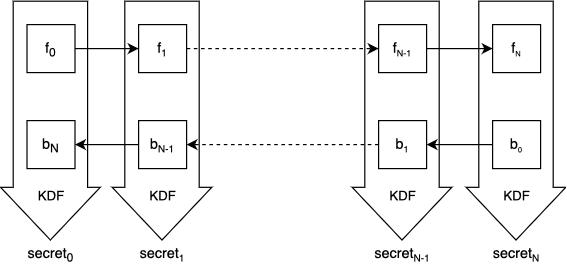
\includegraphics[width=0.8\textwidth]{figures/dkr.drawio.png}
    \caption{Dual-Key Regression (DKR), displaying the forward and backward chains and corresponding sequence of secrets derived through the application of the KDF. }
    \label{fig:dkr}
\end{figure}

A hash chain is a sequence of values
$h_{0}, ..., h_{n}$ which starting from an initial
element $h_0$ progresses by iteratively calculating
a given hash function $H$ on the predecessor,
i.e., given $h_i$, the next element $h_{i+1}$ is computed as $h_{i+1} = H(h_i)$.
Due to the pre-image resistance of the hash function $H$, 
it is computationally hard to find $h_i$ given $h_{i+1}$.
We call an ``interval'' $[a, b]$ a subsequence of elements
of a hash chain starting from index $a$ and ending
on index $b$ inclusive of the chain.
Dual-key regression (DKR) introduced by Shafagh et al.~\cite{USENIX:SBRH20} is a
cryptographic primitive based on hash chains, that
allows sharing a potentially very large interval 
of secrets by only sharing a small state.
Dual-key regression (\cref{fig:dkr}) uses a pair of hash chains,
a ``forward'' and ``backward'' chain, with an additional
parameter $N$ denoting the
upper bound on the maximum length of each chain.
A forward chain is just a hash chain as defined
above, $f_{0}, ..., f_{N}$.
A backward chain instead is a hash chain, of which the
elements are released in reverse order of computation
$b_{N}, ..., b_{0}$, meaning that the element of the chain 
at index $i$ will be the element calculated by $N - i$
iterations of the hash function on the initial $b_{0}$
element. Notice that the DKR upper bound parameter
$N$ is imposed by the fact that elements of the backward chains are taken in
reverse order and the hash function cannot be inverted.
Finally, a DKR secret is calculated by applying
a key derivation function (KDF) that takes as input elements from both chains at the same time corresponding to the same index, i.e.\!
elements $f_{i}$ and $b_{(N - i)}$.
The KDF we will use will be a double-PRF (\cref{sc:DPRF}, \cref{sc:ssf-double-prf}).


\section{Seekable Sequential Key Generators}\label{sc:SSKG}

Seekable Sequential Key Generators (SSKG) are cryptographic objects introduced by Marson et al.~\cite{ESORICS:MarPoe13}.
They are sequential pseudo-random generators (SRG) with additional properties.
A sequential random generator is a stateful pseudo-random generator (PRG)~\cite{cryptoeprint:2017/208}, 
which outputs a fixed-length string for each invocation, 
thus producing a sequence of pseudo-random strings through multiple invocations.
A SRG is said to be secure if its output is indistinguishable from a uniformly random sampled string.
SSKG are SRG with the additional property of being seekable,
meaning that they offer a convenient operation to compute the
element at a certain offset in the sequence from the initial one.
This operation is called \texttt{Seek} and runs in sublinear time.

SSKG are widely used in practice:
the logging service of the \texttt{systemd} system manager,
which is a core component in many Linux-based operating systems,
is using them to power fast verification of arbitrary log entries against tampering.
SSKG are provably (forward-)secure in the standard model, i.e.,
an adversary gets no advantage from learning the current output of the SSKG
while trying to compute the past outputs.
SSKG can be seen as time-efficient alternatives to hash chains (\cref{sc:DKR}),
when the \texttt{Seek} operation is required.
Marson et al.\ propose two constructions: one is based on number theory~\cite{ESORICS:MarPoe13}
and the other one uses a tree-based construction~\cite{ESORICS:MarPoe14}.
The latter suffers a logarithmic space overhead 
compared to the constant space required to store 
only the starting element of a hash chain.
However, in our implementation, we will be using the later tree-based version of SSKG~\cite{ESORICS:MarPoe14}
because it allows seeking also starting from any point in the sequence
instead of just from the initial element.
We discuss the practical details more in-depth in \cref{sc:ssf-sskg}.

\section{Continuous Group Key Agreement}\label{sc:CGKA}

A continuous group key agreement (CGKA) scheme~\cite{C:ACDT20}
allows a long-lived, dynamic, asynchronous group of users to agree 
continuously on shared symmetric secrets.
The shared group secret is recomputed both as users add (remove)
other members to (resp.\ from) the group, and when users periodically
refresh their private secret state. These operations can happen
asynchronously, allowing group members to refresh their 
state without requiring all other members to be online 
simultaneously.
CKGA allows a group of $n$ users to perform the above critical 
operations in $\log(n)$ time,
thus it can be used in practice with a large number of members.
The primitive guarantees post-compromise security (PCS) and forward secrecy (FS):
in case of a compromise in which a user's secret is leaked
to an adversary, the group keys should shortly become private
again through the ordinary protocol state refreshes; the past
group keys remain secure as well.

A first ends-to-ends\footnote{While in communication protocols between two entities (where an entity is commonly referred to as endpoint) we normally speak about end-to-end encryption, in case of a group setting we use the plural form for the term.}
encrypted (E2EE) primitive for an asynchronous group key exchange 
has been introduced by Cohn-Gordon et al.~\cite{CCS:CCGMM18}. The research was conducted to address the scenario of secure group messaging.
In such a case multiple users want to exchange messages, asynchronously and securely
between them, which can be reduced to the problem
of asynchronously agreeing on a shared symmetric key.
The authors presented a way to achieve PCS in such cases.
To this end, they designed the Asynchronous Ratcheting Trees (ART),
which is internally using a Diffie-Hellman tree~\cite{10.1145/1368310.1368347} 
to represent the public and private secrets for each user
and derive a shared secret from them. In Diffie-Hellman
trees, the user keypair is stored in the leaves.
This primitive offers the operations to add and remove members
as well as refreshing a user's own secret efficiently in $\log(n)$ time.
It has been of significant interest in the industry and
has a dedicated working group by the IETF.
The ART construction has been replaced by the TreeKEM
construction proposed by Bhargavan et al.~\cite{TreeKEM}.
In TreeKEM, members are organised in a tree-shaped structure
as in ART, however, the keys stored in the tree for each group
can be any keypair supporting key encapsulation (KEM).
The key advantage of TreeKEM over ART is that
most operations are ``mergeable'':
any device receiving two
concurrent operations will be able to process and execute both of them,
instead of executing one and refusing the other.
Alwen et al.~\cite{C:ACDT20} slightly modified the TreeKEM construction
to achieve \textit{optimal} security in the context of
secure group messaging.
Further refinements for efficiency and security have 
been studied in recent years under different assumptions and threat models~\cite{TCC:ACJM20, SP:KPWKCCMYAP21, CCS:ACDT21, CCS:AHKM22, EC:AANKPPW22, C:AlwJosMul22, C:AlwMulTse23, IWSPA:KEONO23}.

Of particular interest is the family of CGKA protocols called admin-CGKA (A-CGKA).
In this declination of CGKA, a subgroup of the users are admins. 
Admins can perform additional operations that are otherwise disallowed, such as removing other members of the group.

As we will see in \cref{sc:SSF-scheme}, our secure shared folder (SSF) scheme uses A-CGKA as a building block
inside the GKP scheme (\cref{sc:gkp-scheme}).
The specific version of A-CGKA we use, called dual-CGKA, is composed of a CGKA within CGKA to manage the admin state, as proposed by
B{\'a}lbas et al.\!~\cite{USENIX:BalColVau23}.

\section{Messaging Layer Security}\label{sc:MLS}

As already discussed in \cref{sc:CGKA}, a major application of CGKA is in the field of group messaging.
The messaging layer security (MLS) protocol from IETF~\cite{rfc9420},
a standardised protocol for secure group messaging, is indeed 
built on top of CGKA. CGKA is used to agree on a shared symmetric key
to later derive message encryption keys.

CGKA instantiations rely on message exchange
between the members of the group to perform the protocol operations.
Therefore, it is not surprising that most of the implementations
of CGKA come from libraries that also implement the MLS protocol (\cref{sc:CGKA-implementations}).
The messages needed for the CGKA operations are referred to as ``control'' messages in the context of MLS.
CGKA operations are based on a proposal and commit mechanism,
where (multiple) users can propose (multiple) group state updates
through proposal messages and then commit to them through a commit message
sent by one member, referring to a list of previously shared proposals. 
The proposals are of different types and model the operation of adding or removing 
members as well as refreshing a user's secret state, as seen above (\cref{sc:CGKA}).
The commit messages are used to agree and finalise the state updates,
thus helping to synchronize the group state among the members.

The MLS protocol specification also offers an abstract overview of
the component and architecture of a system using it, 
where the concept of a ``delivery service''
(DS) is introduced. The DS is a facilitator component that is used to 
deliver the messages between the members of the group and helps in
synchronising the group state. The DS is assumed to reliably
send the messages to the group members in order, so that the
group is able to advance the CGKA cryptographic state reliably.
However, the DS is not part of CGKA itself,
but it is a necessary component to implement the scheme in practice.
Further, the MLS protocol offers a way to securely exchange ``application messages''
on top of CGKA. The application messages are just opaque payloads
without any predefined structure or semantic, in contrast to the
CGKA control messages.
Application messages are encrypted with a key derived from the shared group secret.

As we will see in \cref{ch:setup}, we use a library implementing MLS and not just CGKA in our implementation of SSF.
We will make use of some additional features from MLS that are not part of CGKA, such as the
aforementioned encrypted application messages,
and take inspiration from the system architecture of MLS for our architecture design.
We discuss the architecture in further details in \cref{ch:setup}.

\section{Secure Shared Folder Building Blocks}\label{sc:SSF}

In this section, we describe the
contributions from~\cite{GKP}
which are going to be used
in the SSF scheme.
We start by recalling the novel security notion for persistent
data called interval access security (IAC) (\cref{sc:iac}).
Then we describe the generalised dual-key regression and the group key progression primitives
(\cref{sc:background-generalised-DKR,sc:gkp-scheme}).

\subsection{Novel Security Notion for Persistent Data: Interval Access Security}\label{sc:iac}

The SSF (\cref{sc:mental-model}) is a new primitive that targets a novel security 
notion for persistent data shared among a dynamic 
group of users: interval access control (IAC)~\cite{GKP}.
The new security notion aims to better and more naturally
capture the minimal security for shared persistent data.

In short, IAC requires that a user can only decrypt data that
is shared in the time frame in which the user is a member
of the group. For data in transit, the data is regarded as
ephemeral and therefore the creation and sharing of the data
itself is naturally bound to the point in time of the exchange,
and to its deletion. Persistent data on the other hand, naturally
outlive the moment in time in which it is shared.
Therefore, the lifetime of data at rest is decoupled from the
lifetime of the user access to the group exchanging the data.
Thus, users that receive access to some data while being the
member of a group, will be able to still decrypt the data
after they lose membership, unless the data is re-encrypted
and the old ciphertext is securely deleted, because data persistence prevents the automatic expiration of the granted access.
In the opposite direction, access to data that has been
shared before the user joined the group could also be granted
to new members.

\subsection{DKR for Unlimited Key Derivations with IAC}\label{sc:background-generalised-DKR}

The SSF construction uses a generalisation of DKR (\cref{sc:DKR}).
The main issue with plain DKR is that it comes with a limit
on the number of derivable keys, which is imposed by the
length of the backward chain. The generalisation aims to
remove this limit.
In the generalised DKR a user can derive a virtually infinite 
sequence of keys.
Each point in the key sequence is associated with one \textit{epoch}, 
which represent the (discrete) time in which the key sequence is advanced.
The term \textit{epoch} can be found also in CGKA and 
MLS~\cite{rfc9420} with similar meaning.
An epoch interval $[a, b]$ is constituted by the subsequence of keys
from epoch $a$ to epoch $b$. We call each key an \textit{epoch key}, and associate
the key with the epoch it belongs to.

We observe that a na\"ive generalisation of DKR allowing
infinite keys to be derived is easily achievable: we can keep the 
forward chain and just start a new backward chain after the 
current backward chain is fully released,
i.e. each $N$ epochs, where $N$ is a single backward chain maximum length.
The state thus grows over time, with the progression of epochs, as the 
user needs to store all the starting backward chains elements. 
Precisely, the space needed is $1 + epoch_{max} / N$, 
where $epoch_{max}$ is the current epoch.

However, by maintaining the same forward chain in the key progression,
a user who has access to epoch interval 
$[t_j, t_{j + c}]$ and $[t_i, t_{i + d}]$, 
where $t_{j + c} < t_i$ and $t_i - t_{j + c} < N$  
can simply derive the keys in the interval $[t_{j + c}, t_i]$, even if 
the user should not have access to them.
To solve this problem, \textit{blocks} can be added on top of DKR.
Blocks aim to restrict access to the keys in either forward, backwards
or both directions by rotating the chains:
\begin{itemize}
    \item A forward block starts a new forward chain, thus preventing an adversary which learnt an element from a prior forward chain from deriving subsequent elements in the collection of the forward chain. 
    \item A backward block starts a new backward chain, thus preventing an adversary which learnt a backward chain element proceeded by such block from deriving previous elements in the backward chain.
    \item A double or full block starts both a new forward and backward chain, thus applying both restrictions.
    \item Finally, an empty block can be used to avoid any chain rotation if the chains are not completely released.
\end{itemize} 
In the example above, starting a new forward chain, i.e.\ adding a forward block,
at epoch $t_i$ would prevent the user that was removed and re-added from deriving the keys in between 
the intervals. Observe that the space complexity to hold the cryptographic
state has a lower bound defined by the maximum length of a backward chain,
but in this case, it grows in the number of blocks. In asymptotic
complexity, the space used is still linear in the number of epochs.\footnote{As a user can add only one block at each epoch.}
Practically speaking, however, inserting a block at each derivation
should be avoided in space-constrained settings.


We will now recall the full generalised DKR scheme from~\cite{GKP}, and we will call it simply DKR from now on. 
A DKR scheme global state is composed of:
\begin{itemize}
    \item A max epoch $epoch_{max}$, which is the current epoch to which the DKR has progressed.
    \item A set of forward (backward) chain elements needed to derive the epoch keys from 0 to $epoch_{max}$, each of them paired with the epoch they belong to.
    \item A maximum size $N$ for the backward and forward chains before a chain rotation is required.
\end{itemize}

We give an informal description of the operations that are provided in DKR:
\begin{itemize}
    \item \texttt{Init}: initialise the state of the DKR.
    \item \texttt{Progress}: on input the global state and a block, progress to the next epoch ($epoch_{max} + 1$) creating new chains accordingly to the block and maximum size $N$. Returns the modified state.
    \item \texttt{GetInt}: on input the global state and an epoch interval $[l, r]$ returns an ``interval state'' which gives access to a sub-interval of the global epoch key interval $[0, epoch_{max}]$. We point out that an interval state is a way to export a partial DKR state to other users.
    \item \texttt{CreateExt}: on input the global state and an epoch interval $[r + 1, b]$, returns
    an extension for these epochs, which can be used to extend an existing interval state $[l, r]$, allowing for a compact representation of the state exported as interval state $[l, b]$.
    \item \texttt{ProcExt}: on input a compatible interval state and extension, returns the
    extended interval state.
    \item \texttt{GetKey}: on input an interval state and an epoch, returns the epoch key corresponding to the epoch or error if the epoch is not in the interval.
\end{itemize}

The \cref{fig:dkr-new-chains} provides a visual representation of the 
state after a \texttt{Progress} operation is executed with different blocks.

\begin{figure}[t]
	\centering
	\includegraphics[width=\textwidth]{figures/dkr_new_chains.pdf}
	\caption{
        From~\cite{GKP}.
		Example of how a progress flag at epoch 4 affects the keys derivable from interval states $(f{0}, b_{5})$ and $(f_{6}, b_{0})$.
		From left-to-right, top-to-bottom: none, new forward chain (forward block), new backward chain (backward block), both new chains~(full block). 
        \label{fig:dkr-new-chains}}
\end{figure}

An instantiation of the DKR scheme, called D[S, F] is proposed in~\cite{GKP},
using SSKG and double-PRF as building blocks. The implementation
details are provided in \cref{sc:DKR-implementation}.
The DKR scheme is used to achieve IAC in GKP (\cref{sc:gkp-scheme}).


\subsection{Group Key Progression Scheme}\label{sc:gkp-scheme}

To implement our SSF construction, we use the group key 
progression (GKP) primitive from~\cite{GKP} and its
instantiation GRaPPA.
This primitive and its instantiation build on top of the previously presented DKR
(\cref{sc:background-generalised-DKR}) and dual-CGKA (\cref{sc:CGKA}) primitives
and takes inspiration from them.
As in CGKA, GKP is used among an asynchronous dynamic group of users
to agree on a sequence of shared group secrets. Those secrets
are derived from a shared state, which is maintained by a
subgroup of the users, called admins. Each key is associated with
an epoch, exactly as in DKR. GKP epochs model
discrete time, in which the group state is changed, through
additions, deletions of users or key rotations as in CGKA.
Only admins are allowed to add or remove other users from the group,
and their cryptographic state might be bigger than the one of
non-admin members.

We informally recall the syntax and operations of GKP from~\cite{GKP}.
As in CGKA and MLS (\cref{sc:MLS}), GKP implicitly rely on a delivery service
to distribute messages among the group members with ordering guarantees.
These messages, as in CGKA, are needed to perform the protocol operations.
The operations of GKP are:
\begin{itemize}
    \item \texttt{InitUser}: initialise the state of a new user.
    \item \texttt{Create}: on input the user state, creates a group owned by the calling user and outputs an updated user state. The creator is an admin of the group.
    \item \texttt{ExecCtrl}: on input the user state, optional arguments, and a command type execute the corresponding action, eventually modifying the state. The list of commands for an admin is:
    \begin{itemize}
        \item \texttt{Add}: add a user to the group with access from the current epoch.
        \item \texttt{Rem}: remove a non-admin user from the group.
        \item \texttt{RotKeys}: rotate the key material of the entire group.
        \item \texttt{AddAdm}: add an existing member to the admin group and share the complete admin state.
        \item \texttt{RemAdm}: remove an admin user from the admin group.
        \item \texttt{UpdAdm}: refresh the state of the calling admin. 
    \end{itemize}
    The commands for a non-admin user are:
    \begin{itemize}
        \item \texttt{UpdUser}: refresh the state of the calling user.
    \end{itemize}
    Each of the commands above produces a control message and/or a welcome message, to be sent to the other members of the group through the delivery service.
    \item \texttt{ProcCtrl}: on input the user state and a control message, process the control message, evolve the epoch accordingly and return the updated user status.
    \item \texttt{JoinCtrl}: on input the user state and a welcome message, process the welcome message to join the group. Return the updated user state.
    \item \texttt{GetEpochKey}: on input the user state and an epoch, derive the corresponding epoch key and return it.
\end{itemize}

In a correct GKP, all parties, i.e.\ members and joining users, which process a correct
sequence of welcome and control messages, should be able to derive the same keys
for each epoch they are given access to. The mathematical syntax assumes
no global state is stored outside the clients, however, this assumption is challenging
in practice as we detail in \cref{ch:ssf},
especially refer to \cref{ssc:GKP-client-middleware,ssc:delivery-service}.

The construction GRaPPA instantiates GKP using dual-CGKA~\cite{USENIX:BalColVau23}
and DKR \cite{GKP} as building blocks to achieve IAC (\cref{sc:iac}) for the shared group epoch keys.

IAC can be enforced by properly adding blocks in DKR at membership
changes, to prevent new members from deriving past secrets (as in the previous detailed example)
as well as old members to derive future secrets. See \cref{fig:gkp-iac} for an example.

\begin{figure}[t]
	\centering
	\includegraphics[width=\textwidth]{figures/gkp-meta-figure.pdf}
	\caption{
        From~\cite{GKP}.
        Group key progression (GKP) example built on dual key regression (DKR) to achieve interval access control
        (IAC) for shared persistent data.
        \label{fig:gkp-iac}}
\end{figure}

The implementation details are provided in \cref{sc:GRaPPA-implementation}.
We provide an overview of the state of GRaPPA users, which we derive from the protocol description and pseudocode in~\cite{GKP}. 
Note that the cryptographic state of an admin contains the cryptographic state of a member as described below.
Members maintain the following cryptographic state:
\begin{itemize}
    \item A user identity.
    \item The state of a member CGKA group (from dual-CGKA), $CGKA_M$.
    \item The interval state $int$ to which they have access to (exported from D[S, F] construction by admins, see \cref{sc:DKR}).
\end{itemize}
Admins additionally store and have access to:
\begin{itemize}
    \item The state of an admin CGKA group (from dual-CGKA), $CGKA_A$.
    \item The DKR state instead of just the interval state $int$, where the current epoch $epoch_{max}$ is the current epoch of the group in GRaPPA.
\end{itemize}


Note that we simplify our description here by not explicitly mentioning the current epoch as part of the state of a user:
for admins, this is implicitly part of the DKR state, while for members it is implicitly part of the interval state.
In contrast, each CGKA group state includes a current epoch of the group,
which diverges from the GRaPPA epoch, as it is determined by changes in
the CGKA group state composition and by user secret refreshes internally in the
CGKA group itself only. State management is a critical aspect 
of the implementation, and will be discussed in detail in \cref{sc:state-sync-rollbacks}.


\chapter{System Design}\label{ch:setup}

In this chapter we discuss the overall system design of the project.
First, we provide an architectural overview
of the system and the various components in \cref{sc:architectural-overview}.
We then discuss the requirements of the system from the user's point of view
(\cref{sc:real-user}), from the cryptographic point of view
(\cref{sc:abstract-to-real}) and from the developer's point of view
(\cref{sc:developer}). We highlight the importance
of taking into account all points of view and stress the 
relevance of considering the real-world
user for the choice of technologies in the implementation. 

After laying out the requirements, we discuss the various
components of the system, detailing for each of them
the technology we use. In-depth technical
discussion and technology surveys are provided
to motivate our final choice when required, and we believe
that this is of great interest to the practitioners
that want to implement cryptographic systems with 
a similar technology stack.\footnote{The term ``technology stack'' (or tech stack) generally refers to the set of technologies used together to build a software product.}
However, the reader should feel free to safely skip
them, as they are not strictly necessary to understand 
the rest of this work.

We only discuss common
pieces to both the baseline and the SSF implementation
in this chapter. Most of the system is
shared between the two implementations, to allow
for easy comparison and benchmarking.
The specifics of each implementation are instead discussed respectively in \cref{ch:baseline,ch:ssf}.

\section{Architecture Overview}\label{sc:architectural-overview}

In figure \cref{fig:architecture} we provide a high-level system architecture overview.
We use different colours to highlight different components of the system, grouping
by frontend, backend, relational databases and cloud components.

\paragraph{Client} The SSF client is a web application that
runs in the browser. The client is used by the user to interact with the system, and performs the cryptographic
operations needed to access, store and retrieve files 
from the shared folders the user has access to.
Although in the \cref{sc:SSF-scheme} we only model one folder,
in practice the system supports multiple ones.
We imagine the final version of the user interface (UI) to
be similar to the one of Google Drive or Dropbox, where
the user can see the shared folders and navigate inside each
of them to see a list of files stored in each of them.
The UI is out of scope from this project, due to
time constraints (\cref{sc:client-overview}), we will
instead provide a command line interface (CLI) client
as MVP.

\paragraph{PKI} The system needs a PKI to manage the identities
of its users. We assume a corporate environment, where
an internal identity provider is available. The PKI server
is a simple certificate authority (CA) which is trusted
by the clients, and issues certificates to users of the system.
The CA certificate is generated once and embedded in the client
code to allow for the verification of other users' certificates.
All the certificates are stored in a relational SQL database \texttt{pki}.

\paragraph{SSF Gateway and DS}
The SSF Gateway server is the main backend component of the system.
The same server will be used also to implement a delivery service (DS) (see \cref{sc:MLS} and \cref{ssc:delivery-service}).
These are two different components in abstract, but in practical terms, 
we will see that they share some state (\cref{ssc:delivery-service}).
The SSF Gateway, or simply Gateway, is responsible for the
creation of the shared folders (\cref{sc:SSF-scheme}) and the management of user access
to them. The shared folders are stored in a relational SQL
database \texttt{ds}, together with the users access control lists (ACLs).
Since different cloud storage providers offer different APIs,
the Gateway is responsible for abstracting away the specific
vendor and providing a common API to the clients.
Through the Gateway, files can be uploaded and downloaded 
from the cloud storage provider, which is hidden from the client,
as can be seen in \cref{fig:architecture}.
We can imagine, that the Gateway would constitute the main
server of a company offering a service for secure file sharing.

\begin{figure}
    \centering
    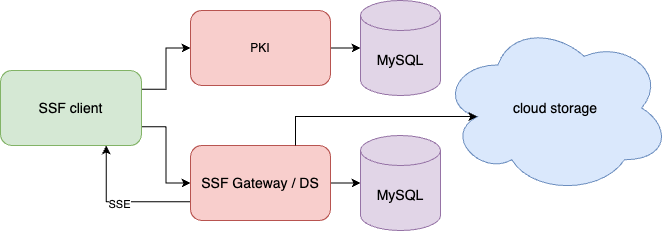
\includegraphics[width=0.8\textwidth]{figures/architecture.png}
    \caption{System Architecture Overview: The main components of the system are shown with the dependencies between them.}
    \label{fig:architecture}
\end{figure}

\section{High-Level Practical Requirements}\label{sc:requirements}

After this initial very high-level overview of the system, we
now move on to discuss its requirements instead and continue with a more
detailed explanation of the components of the system in the following sections.
This should motivate some of the choices we made in the architecture,
and be the background for the following detailed description.

\subsection{Starting with the User in Mind}\label{sc:real-user}

A goal of this thesis (\cref{sc:summary-of-contributions})
is to create an MVP. To this end, we start by asking ourselves,
as users of the system, what do we want from it?
\footnote{The study of the use cases and situations from a product 
point of view in industry is normally done through so-called ``user stories''.
User stories as sentences that try to summarise a workflow from the
point of view of a user. They have the following structure:
``As [a user persona] I want [to perform this action] so that [I can accomplish this goal]''.}
Our exploration is limited in time therefore we want to simplify
our requirements to the minimum necessary to run the system
in a real-world setting, 
but still with a customer-centric\footnote{To be customer-centric is a famous Amazon core approach. Indeed, Amazon has a leadership principle called ``customer obsession''~\cite{AmazonLeadershipPrinciples}.}
approach, leaving the possibility to iterate over the initial implementation~\cite{ries2011startup}.
We stress that we do not want to develop just a proof-of-concept of the protocol,
but something practically deployable and scalable to a large
amount of users.

As users, we expect to be able to access 
cloud systems from any device that can navigate online.
This is indeed a core minimum requirement for any modern
cloud storage solution for market adoption.
We also think this is a challenge that is worth exploring
in the context of SSF to understand if the underlying
schemes (\cref{ssc:GKP-client-middleware} \cref{sc:background-generalised-DKR})
are feasible and applicable for real use cases.
Normally, such ubiquitous access to cloud storage solutions,
is through a web interface.
This in turn means that we need to run our code (at least a part of it) 
in the browser of the user.

Other user expectations include updates and changes to uploaded files.
Further, we expect our system to provide multi-tenancy,
meaning that we handle multiple groups of users at the same time.\footnote{Note that each shared folder is in a one-to-one relationship with the group of users that have access to it.} 
Another side of the multi-tenancy aspect is that a 
single user could be part of multiple such groups at once. 
However, we point out that the SSF scheme (\cref{sc:SSF-scheme}) 
itself is designed for a single shared folder at the time.
Indeed, the underlying primitive GKP (\cref{sc:gkp-scheme}) focus 
on one group at a time in an isolated execution environment:
it is therefore up to our implementation to fill this gap.

We highlight that all major (non-E2EE) file sharing solutions available today meet the above requirements.
Therefore, we claim that these requirements and expectations should be met by any serious attempt to create a new cloud storage solution, including the implementation of the SSF scheme.\footnote{A notable exception is Apple's Advanced Data Protection, which is not accessible via web browser. This is partially thanks to the high level of integration of Apple hardware and software.}

\subsection{Cryptography: from Math to Real Execution Environments}\label{sc:abstract-to-real}

Before writing any code, we need to choose the right 
programming language that targets the execution environment
we want to run the code in.

As seen in \cref{ch:background}, the SSF scheme (\cref{sc:SSF-scheme})
uses some advanced cryptographic primitives:
\begin{itemize}
    \item continuous group key agreement (CGKA) (\cref{sc:CGKA})
    \item seekable sequential random generators (SSKG) (\cref{sc:SSKG})
    \item dual-key regression (DKR) (\cref{sc:background-generalised-DKR})
    \item group key progression (GKP) (\cref{sc:gkp-scheme})
\end{itemize}
Implementing these primitives from scratch could in itself
be a complex, time-consuming and error-prone task, especially for CGKA.
It is therefore important to use libraries when available
to deliver reliable implementations.

In our execution environment 
we need support for all cryptographic operations
needed both by the primitives above and by simpler
cryptography which is normally exploited and assumed to exist. 
To be more precise we require:
\begin{itemize}
    \item Secure random number generation.
    \item Availability and constant time execution of the cryptographic operations underlying the constructions we implement, both for the baseline and the SSF scheme.
    \item Memory safety.
\end{itemize}
The above requirements are needed to avoid security
issues in the implementation. For example, a non-constant
time execution of the cryptographic operations could
lead to timing attacks. 
However, during our implementation work, 
we found that in major runtime
environments, such as the browser, 
support for the cryptographic operations normally
used to instantiate cryptographic primitives is not always available.
This might lead to the usage of custom implementation,
where such guarantees are impossible to provide because
of the lack of low-level control on the execution environment.
We detail such findings throughout the rest of the thesis,
and summarise them among other engineering issues in \cref{ch:gaps}.

\subsection{What does the Developer need?}\label{sc:developer}

As developers, we face the challenge of implementing a full
system in a very short time frame and with limited resources.\footnote{To be more precise, the whole implementation has been conducted by only one person in less than six months.}
We want to reduce the possibility of errors and bugs
as well as the complexity of maintaining the integration between
different components.
Sometimes, just a small change in the protocol can lead to
hundreds of lines of changes in the code.
Even more, we want to be able to easily prototype, i.e.\ test
out different ideas coming from the theoretical side
or different engineering solutions.
However, changing requirements during the implementation
and updating the system accordingly can take up months of work
if the setup is not properly done to allow development agility.
We will see how this is achieved in the description of the various components.


\section{The PKI}\label{sc:PKI}

This section presents the PKI server implementation from the architecture overview (\cref{sc:architectural-overview}).

Recall from \cref{sc:mental-model} that
we need a Public Key Infrastructure (PKI) to implement the SSF scheme.
Papers in cryptography normally assume the existence of a PKI,
which solves the problem of mapping identities to cryptographic keys.
Since we want to develop the code easily, and the PKI itself
is not the core problem we are focusing on, we want to rely on existing
solutions.
A common standard way to manage identities is through X509 certificates~\cite{rfc5280}.
To implement this solution, we need to have a Certificate Authority (CA)
to distribute the certificates.
Our MVP target use case is a company or organization. 
Thus, we can assume to have an internal identity provider.
We implement a simple CA, with an endpoint for users
to register and one to fetch users' certificates. 
Users send certificate signing requests to be signed by the CA to register.
The CA certificate is bundled with the client code, to
allow the verification of other users' certificates.
The endpoints of the PKI are secured through TLS,
while the SSF Gateway will use mutual TLS (\cref{sc:ssf-proxy-server}).
We highlight that this PKI server implementation is not meant for production use:
for instance, we implement our CA purely in software, while a production
version would need to support hardware security mechanisms to
store secret key material.


\paragraph{Implementation Details} 
The PKI server is implemented in Rust, using \texttt{Rocket}~\cite{Rocket}
framework for the server and \texttt{sqlx} driver to interact
with the MySQL database.
In the early exploration of the project, we tried
to use other Rust web development frameworks,
such as \texttt{Actix}~\cite{Actix} and \texttt{Warp}~\cite{Warp}.
However, we found that \texttt{Rocket} was the most
suitable for our needs (see also \cref{sc:ssf-proxy-server}),
thanks to its support for retrieving the certificate
from the request when mTLS is used.
As we want to minimise the development overhead, we
try to reuse frameworks and libraries as much as possible. 

For local development, 
the database runs in a Docker container, which allows
for easy setup and teardown.\footnote{Docker is a lightweight virtualization technology. Docker containers are equivalent to lightweight virtual machines, but access the host's kernel rather than perform full CPU and IO virtualization.} 
The database is initialised with the script \texttt{sql/pki\_database.sql}.
It is important to have the ability
to easily reset the database to a fresh state 
while developing and testing the system.
The commands to start and stop the container are provided
in the top level \texttt{README.md} of the project.

The code is available in the \texttt{pki} crate
of this project, in \texttt{services/pki} folder.\footnote{``Crate'' is the name for a Rust package.}
The server exposes a simple API
to issue certificates to users. 
When issuing a certificate, validation is not performed
on the user identity, as this is out of scope for the MVP.
A client can send a certificate signing request (CSR)
to the server and receive a signed certificate in return.
The signing algorithm is ECDSA using P-256 curves and SHA-256 hashing
as described in~\cite{rfc5758}.
The code to construct the CSR and issue certificates, as well as 
verify them is available in the Rust crate \texttt{common},
which is shared among servers and clients (\cref{sc:client-overview}).
We provide unit tests for the library and expose simple bindings (\cref{sc:browser-runtimes}) to be
called from JavaScript in the client (\cref{sc:client-overview}), check the \texttt{README.md}
of the crate for details. All the exposed functionalities are stateless.

The certificates are stored in MySQL ``pki'' database, and the CA
certificate is copied and embedded in the client code to allow
for local verification of other users' certificates.
The server exposes an endpoint to fetch the
CA certificate, which can be used by clients to
refresh the embedded CA certificate.
Further, an endpoint to fetch users' certificates providing the email of the target user is available.
The description of how to compile and start the server is
provided in the \texttt{README.md} file of the \texttt{pki} crate.
The server is exposed locally at \texttt{\url{https://localhost:8000}}



\paragraph{OpenAPI Specification}
The server API is available in OpenAPI
specification format~\cite{OpenAPISurvey} 
which is generated automatically from the code using
\texttt{utoipa}. Each server endpoint code is
annotated through the library annotations, with the description
of the endpoint, parameters etc. \texttt{utoipa} is then
able to generate the OpenAPI specification in YAML format.
We store the generated file in \texttt{openapi/pki-openapi.yaml}.
We provide an executable written in Rust to perform the generation
through \texttt{utoipa} and regenerate the \texttt{.yaml}
file when the server endpoints are modified.
The OpenAPI specification is then used to generate the
code in TypeScript, which is used by the client to interact
with the PKI server (\cref{sc:client-overview}), thus sparing
the developer from writing thousands of lines of code and keeping them up to date, 
as well as reducing the possibility of errors in the client-server interaction. 
The guide on how to use the executable can be found in the \texttt{README.md}
of the crate.
While the server is running, the OpenAPI specification can be
accessed nicely through the Swagger UI from the browser, 
by visiting the page \texttt{\url{http://localhost:8000/swagger/UI}}.

\section{Cloud Storage: from an Abstract Model to Real Systems}\label{sc:cloud-storage}

This section provides the necessary background on cloud storage,
aiming to provide the reader with a first understanding of the challenges
we encounter when dealing with real cloud storage system
as compared to the abstract model we can find in academic papers.
Seemingly intuitive properties of cloud storage, such as faithful deletion of files from honest
providers, uniform APIs, and guaranteed success of read and write operations do not stand the test
of reality.
This creates gaps between abstract protocols and their concrete implementations
which we will expand on in more detail in the next sections,
where we will use the cloud storage provider to store the shared folders' contents.
This is particularly relevant for the implementation of the
SSF Gateway server (\cref{sc:ssf-proxy-server}).

\subsection{Assumptions}\label{scc:cloud-storage-assumptions}
In the cryptographic research, cloud storage systems are abstracted away by assuming
that some operations are available to write and read data to a virtually
infinite always available storage system.
This is a well-founded assumption, as a cloud storage provider
will normally provision new hardware as needed (in advance) to accommodate the
increased capacity request~\cite{AzureBlobStorage}.

Deletion of files cannot be assumed to be secure, meaning that even a storage provider that is
not malicious is not guaranteed to faithfully delete and completely delete data upon request.
We motivate this assumption with the following facts:
\begin{itemize}
    \item Cloud providers state in their Service Level Agreement (SLA) that
    the service is guaranteed to be up and running for more than a certain percentage of time or a refund is paid out to the clients.\footnote{e.g.\ Amazon Simple Storage Service (Amazon S3) starts to pay a refund to clients when the monthly uptime percentage is less than 99.9\%}
    The SLA also assures the durability of content uploaded is at least a certain percentage.\footnote{As an example again, Amazon S3 is designed for 99.999999999\% durability}
    To meet the SLA, cloud providers replicate the content. The content is replicated at least (normally) 3 times, and possibly in different geographical zones, to protect against widespread failures~\cite{AzureBlobStorage}.
    \item The content is automatically monitored and re-replicated in case some storage devices are failing.
    \item It is well known that in most case deleting a file from a disk does not delete the content but only marks that disk space as free without zeroing out the bits~\cite{manRM}.
    \item The replicated storage could be eventual-consistent, 
    meaning that in case of a network partition the two 
    parts of the system continue to work independently. 
    In this setting, if, while the network is partitioned a side of the storage receives a deletion operation 
    for a certain file, upon restoration,
    the nodes still owning the data would try to replicate 
    them to the other side.
    Therefore, instead of deleting the information, 
    the distributed data store creates a (usually temporary) 
    tombstone record to keep track and eventually perform 
    the deletion on all other nodes as well upon reconciliation.
\end{itemize}

We also highlight the following issues when working with
real cloud storage systems, which will be discussed in the
follow sections:
\begin{itemize}
    \item Cloud storage technologies are of many types.
    Different providers can differ in the way they
    offer similar services.
    When setting up the project we need to choose the right
    technology to use. We also need a way to
    abstract away the specific vendor for the storage
    to ensure that our solution is easily portable.
    We introduce and discuss on technology of choice in (\cref{ssc:object-storage})
    \item The cloud storage system is not accessible freely
    by clients. Access to cloud resources is
    granted by cloud providers upon registration and payment
    for the service. A system implementing the SSF scheme
    needs to deal with this aspect and its implications
    on the system design and in terms of security (\cref{sc:cloud-storage-access-and-billing}).
    \item Abstracting the cloud storage system as read/write
    operations on a virtually infinite storage system does
    not capture the complexity of concurrency and consistency
    issues that arise in real-world systems. Although this
    might not be relevant for security in the SSF scheme,
    it is relevant for the correctness of the system and
    security properties normally expected by users (\cref{sc:ssf-file-changes-sync}).
\end{itemize}

\subsection{Object Storage}\label{ssc:object-storage}
As we need to store the shared folders' contents in the cloud,
we surveyed the available storage solutions.
Cloud providers offer different products,
each with different characteristics. The main file
storage solutions on the market can be divided into
file systems, object storage and databases.

Databases are not needed in this case,
as we do not want to analyse the data stored in
the cloud. Files are encrypted by the client
before the upload.

File systems offering could be used to implement
our shared folders. However, the SSF scheme does not
assume any hierarchy inside a shared folder.
Also, file systems API is rather more complex
than the abstraction that is considered by the
theoretical construction. File storage is also offered
at more expensive prices than the alternative object storage solution.

Object storage solutions provide
very simple API that allows to store and retrieve
objects in a flat namespace.
The name object storage derives from the fact that this type
of storage does not handle files and file hierarchies 
as we would expect in a file system. Instead,
files are grouped as a plain list of objects,
inside a top-level namespace, called a bucket.\footnote{The name is borrowed from Amazon S3, the first such system.}
This type of storage has all the characteristics that are assumed
in academic papers and
for the SSF scheme (\cref{sc:SSF-scheme}).
Stored files are called objects and have the following characteristics:
\begin{itemize}
    \item An object can be big (e.g.\ in Amazon S3 up to 5 GB in a single chunk).
    \item Objects generally can only be written all at once and updating or deleting them creates new versions of the entire data. A special case is append-only objects, which can be extended with new data without rewriting the whole object each time, but still disallow in-place modifications of the existing content.
\end{itemize} 

We do not require the ability to update the content of the files in place,
as the file is always sent encrypted by the client. 
The server has no visibility on the content. 
Updating the file
would always mean completely rewrite it.
Object storage solutions are normally cheaper than the alternatives
and are designed to be highly available and durable.
The cost is really important when considering the implementation
of a real-world system.

Examples of object storage solutions are Amazon Web Services (AWS)
Simple Storage Service (Amazon S3), Microsoft Azure Blob Storage, Google Cloud Storage (GCS).

In our implementation we will use Amazon S3, as it is the most
popular object storage solution, and it is widely used in the industry.
During development to avoid incurring costs, we will use LocalStack~\cite{LocalStack}
to emulate Amazon Web Services locally on our machine. The availability
of such a development tool was also determined in the choice
of the cloud storage provider for testing. LocalStack
runs as a Docker container.

To avoid vendor lock-in, we will abstract the cloud storage provider
and allow for multiple storage solutions to be used.\footnote{Vendor lock-in indicates the condition where a customer is dependent on a vendor for products and services, and cannot move to another vendor without substantial costs.}
We discuss the implications of this choice in \cref{sc:cloud-storage-access-and-billing}.
The implementation details for the abstraction are given in \cref{sc:ssf-proxy-server}.


\subsection{The Need for a Gateway to the Cloud}\label{sc:cloud-storage-access-and-billing}
One of the main goals of the SSF scheme is to provide
end-to-end encryption (E2EE) of the data stored in the cloud.
This means that the data is encrypted by the client before
being uploaded to the cloud storage provider.

In the scheme, we consider only two actors:
clients and the cloud storage provider.
However, notice that we cannot implementation
our scheme only in the client, as we observe that:
\begin{itemize}
    \item We still want to provide non-cryptographic access control. 
    Although availability is normally kept out of scope in cryptographic 
    protocols such as CGKA, MLS, GKP etc., it is expected by users
    in any real-world system. We can not just dismiss the questions about
    what happens if a malicious user tries to download all the encrypted
    data from our shared folder or if the data is overwritten by external
    actors not part of the group. We also point out that although 
    data is E2EE, thus unreadable from users not part of the group,
    the read operations are still billed by the cloud storage provider.
    Users will expect their data to be durable
    and available. The shared folder should be protected from
    denial-of-service attacks. 
    A recent empirical study from K. Izhikevich et al.~\cite{izhikevich2023using},
    shows that there is a strong interest
    in compromising publicly accessible data storages,
    especially when relatable to commercial entities.
    \item We want to abstract away the details of the storage system.
    A service offering secure file sharing should not force the users
    to register with a specific cloud storage provider. However,
    any cloud service requires an account to be created to access it.
    \item Payment for the storage is required by the cloud storage provider.
    The payment of the storage provider should be handled transparently to the users of the system. Users of the system should only pay
    for the usage of the system, not for the storage itself. The storage
    cost will be included in the billing of the system among the members
    of a shared folder.
\end{itemize} 

To solve the above problem, we write a minimal wrapper component around
the cloud storage providers, called the SSF Gateway, which will manage
access to the cloud storage provider. The Gateway acts as a proxy
between clients and the underlying storage provider, as shown in
\cref{fig:architecture}. We discuss the implementation of the
Gateway in (\cref{sc:ssf-proxy-server}).


\section{SSF Gateway Server}\label{sc:ssf-proxy-server}

In this section, we discuss the implementation of the SSF Gateway server 
(\cref{sc:architectural-overview}). This server is responsible for the
management of the shared folders and the access control.
It also abstracts away the communication with the cloud storage provider
and provides synchronization among members of a shared folder.
We discuss the implementation details
of the server, the technology stack used and the
integration with the cloud storage provider.

\paragraph{Implementation Details}
The technology stack of the SSF Gateway server
is similar to the PKI server (\cref{sc:PKI}).

The code can be found in \texttt{services/ds} folder.
See the \texttt{README.md} file in the folder for instructions
on how to compile and run the code.
Locally, the server is exposed at \texttt{\url{https://localhost:8001}}.
Integration tests are provided in the \texttt{tests} folder,
where we test the server API and the access to the 
MySQL database and the cloud storage.
As in \cref{sc:PKI} we use Docker to run the MySQL database.
Initialization scripts are provided in \texttt{sql/ds\_database.sql}.
To run the tests, refer to the instructions in the \texttt{README.md}.

The code is written in Rust, using \texttt{Rocket}~\cite{Rocket}
framework for the server and \texttt{sqlx} driver to interact
with the MySQL database.
The Gateway interacts with the cloud storage provider
through the \texttt{object\_store} crate, a Rust library
that abstracts away the specifics of each cloud storage provider.
We can therefore easily switch between different providers, by
just changing the configuration file of the server (\texttt{DS\_Rocket.toml}).
Recall that to test locally, we use Amazon S3 and
LocalStack (\cref{ssc:object-storage}).

\paragraph{Authentication and Authorization}
Building on top of X509 certificates (\cref{sc:PKI}), we use
mutual TLS (mTLS) to 
secure communication between the clients and the server.
While TLS only verifies the server certificate,
in mTLS the client also provides a certificate to the server
for authentication.
This way, we greatly simplify development. Indeed, we 
avoid introducing any other Authentication
protocol such as OAuth2 or usage of JWT tokens. 
The server expects the client to provide a certificate
to authenticate itself, which must be signed by the
PKI server (\cref{sc:PKI}).
The path to the CA certificate is configured in the
server configuration file (\texttt{DS\_Rocket.toml}),
together with the certificate and private key of the
Gateway server itself. Rocket provides support for
mTLS, and in particular to extract the client
certificate from the request. The certificate is then
made available to the server code handling the request.
We parse the client certificate and extract the email
of the user from it. This email is used to authenticate
the user and to check the access control list (ACL)
of the user to shared folders when the user tries to
access them.

\paragraph{Database}
Our server is multi-tenant, meaning that it can handle
multiple shared folders at the same time.
The database is kept minimal to provide the necessary 
access control functionalities and power the
API of the server. In particular, the server has access to
and stores the list of members that can access a shared folder.
However, notice that the server could infer the list of members
from the access pattern to the folders or files
in the cloud storage.


\paragraph{Endpoints}
The server exposes REST APIs to: register the requestor to the system,
list all the users in the system,
create a shared folder for the requestor,
add a user to a shared folder,
remove the requestor from a shared folder,
list all the folders a user has access to,
upload (download) a file to (from) a shared folder.
As discussed above the server always extracts the identity,
i.e., user email, from the client certificate to authenticate
and authorize the user to perform the operation.
All endpoints apart from the one to register the user
to the system, that writes data in the database,
will trigger a database transaction 
to ensure a consistent state of the system while
handling the request to authorize the
user consistently.

\paragraph{Access Control}
Recall that the server stores the list of users which have access to
a folder. 
The server disallows members from removing other members from a folder and only allows self-removal operations.
This is done only at the database level, but
in the SSF scheme, admins can remove other users'
access to the folder content, through cryptographic means
(\cref{sc:gkp-scheme,sc:SSF-scheme}).
The server protects from denial-of-service attacks,
where a member of a folder could remove other members,
thus negating the access to the data, even if the other
members still have the decryption keys.
We stress that this only applies to non-cryptographic
access control as performed
by the server.
This choice does not affect the security of the system,
as the data is E2EE.
In the simple baseline protocol,
we assume that users are not allowed to
remove another member from a shared folder (\cref{ch:baseline}).
In the SSF scheme implementation (\cref{ch:ssf})
the security of the new data uploaded to the folder
after a member is removed or leaves the group
is cryptographically guaranteed by the GKP scheme (\cref{sc:gkp-scheme})
Notice that a user who is removed could still
have legitimate access to the data for which
it has the decryption key(s), which further motivates
our choice at the access control level. Indeed, we want
to still allow the user to access this data after the removal
from the group sharing new secrets.


\paragraph{Synchronize Concurrent Writes to the Cloud Storage}\label{sc:ssf-file-changes-sync}
The \texttt{object\_store} library, which
we use to communicate with the cloud provider,
also handles concurrent writes
to an object (\cref{ssc:object-storage})
through optimistic concurrency control:
when trying to update an object,
the server also sends to the cloud storage the
ETag (version)
of the object version the update is made upon.
If the version is different, 
the cloud storage will reject the update.
However, Amazon S3 does not support this 
behaviour as an atomic operation. 
The server itself in this case would need to read the version,
check and then write the new object.
Between the read and the write operation,
there would be no guarantee that the version was not changed.
Therefore, the library uses shared locks held in an Amazon DynamoDB 
table~\cite{objectStoreCommitProtocol} when targeting Amazon S3.\footnote{Amazon DynamoDB is a key-value eventual-consistent database, which offers really low latency and high availability.}
Note that readers can always concurrently access the objects. 
Although normally abstracted away in the cryptographic
literature, the synchronization of concurrent writes
influences the communication protocol
between clients and the server when uploading
files to the shared folder 
that will be discussed in
\cref{sc:metadata-synchronization}
and \cref{sc:ssf-file-encryption}.

\section{Allow the User to Interact with the System: the Client(s)}\label{sc:client-overview}

This section discusses the client side of the system,
called SSF client in the high level architecture (\cref{sc:architectural-overview}).

\paragraph{The Scope of the MVP Client}
As seen in \cref{sc:real-user}, 
we want our client to ultimately be a web application,
running in a browser.
However, for the first development iteration, we want to
remove the development burden of building a UI, which is
a time-consuming task. We instead want to focus on the
implementation of the cryptographic constructions (\cref{ch:background}). 
Still, we want to implement them is such a way so that we
will be able to just run the same code inside the browser,
which is the final target execution environment.
The browser client setup is showcased
in the \texttt{www} folder. Interested practitioners
should check the respective \texttt{README.md} file
for the instructions on how to compile and run the code.

\paragraph{Development Agility} 
To test out the implementation (\cref{sc:developer}), 
and provide the users of our system
with the first MVP version, we develop a
command line interface (CLI) client.
Internally, the CLI will use the cryptographic constructions'
implementations. This part of the code will be tested to be executable
inside the browser to ensure portability and allow a subsequent fast
migration to the final UI. The code for the CLI
can be found in the \texttt{ssf-client} folder.

\paragraph{Code Portability}
Since we want E2EE guarantees (\cref{sc:SSF-scheme}), the protocol execution needs to happen
in the client device of the user.
This implies that we need to investigate the various options
in terms of runtime support in the browser (and in the CLI runtime) 
to check if we can also execute all required cryptographic 
operations (\cref{sc:abstract-to-real}).
Our code portability requirements brought us interesting findings on runtime compatibilities, detailed in \cref{sc:Web-Crypto-API-implementations:-non-standard-behaviours}
and \cref{sc:MLS-enhancements}. As noted in these sections,
subtle differences in the runtime environments
make the implementation of portable and secure 
cryptographic software a challenging, or impossible, 
task.

\paragraph{Execution Runtimes} 
Refer to \cref{sc:browser-runtimes} for an in-depth survey about browser runtimes.
We do not only explore the browser setting, but also explore
the portability of the code from and outside the browser.
Libraries written in other languages could be ported and used in the implementation.
In short, two runtime environments are available in the browser:
\textbf{JavaScript} (JS), mostly used in web development, and \textbf{WebAssembly} (Wasm),
a newer execution platform, normally the right choice to achieve better performance
and to port code from other languages to the web. Wasm is normally
used in combination with JS, as it cannot interact directly with
the web page as well as with the browser APIs. Furthermore, 
as mentioned above, we also want to use our code to first build a CLI.
Node.js is a natural choice to run JS and Wasm outside the browser,
for our portability needs, as it is based on the same 
JS execution engine as Chrome, V8.
Instead of developing directly in JS, we implement in TypeScript (TS),
a statically typed superset of JS, to avoid common JS pitfalls.
For a full, in-depth explanation see \cref{sc:browser-runtimes}.

\paragraph{Cryptographic Support and Libraries}
In \cref{sc:webcrypto-api} we describe the cryptographic API
available in the browser and its limitations. Since we need to use
such API to perform the cryptographic operations, we will use JS
as the main runtime environment.
Notice that the same API is also implemented and supported in Node.js.
We survey the available 
implementation to date of CGKA and MLS
to the best of our knowledge (\cref{sc:CGKA-implementations}).
To use the best available
and browser-compatible implementation of these cryptographic
primitives we need to integrate Rust code compiled to Wasm, which is
called from JS in our client code. We remind the reader that
Rust is a memory-safe language.
Thanks to its memory safety guarantees and performance,
as well as its expressive type system which prevents many errors already at compile time,
it is a good choice to write cryptographic code.
The library of choice is mls-rs~\cite{AWSMLSGroup}, developed by AWS Lab, 
and open source on GitHub.\footnote{AWS Lab is a research branch of Amazon Web Services (AWS). GitHub is a famous git-based source code-sharing platform. The term ``open source'' refers to the fact that the code is publicly available and, as we will see, anyone can read and modify it. Normally, the code is distributed under a licence, so usage might be restricted.}
The library is licenced under MIT and Apache version 2.0, both
permissive licences that allow for unrestricted commercial use of the code.

\paragraph{Certificate Validation}
As we are already using the Rust to Wasm toolchain, 
we will also use some Rust code shared
with our servers to check certificate validity in the client.
This code is provided in \texttt{src/common} as a Rust library
with both native and Wasm compilation targets (\cref{sc:PKI}).
This reduces the amount of code duplication and interoperability
issues between the client and the server. Interested practitioners
should check the \texttt{README.md} file for the
instructions on how to compile the code and the configuration
in \texttt{Cargo.toml} to allow both native and Wasm compilation
targets. We use conditional
compilation to configure how dependencies are imported
given a compilation target. To allow for local verification
of other users certificates,
we embed the CA certificate in the client code.
For testing purposes, we generate also the servers' certificates
from our testing CA.
We also install the servers' certificates in the client code,
to allow for the verification of the servers' identities
in the Node.js CLI, by including them in our HTTPS calls.
See the \texttt{ssf-client/src/protocol/authentication.ts} file.
To call the servers from the browser client,
we need to install the servers' certificates in the OS
certificate store, so that the browser, while connecting 
using the HTTPS protocol, can verify the servers' identities.

\paragraph{Code Generation}
To interact with the servers, we need to write code to
call all the endpoints they expose.
Instead of writing the code manually, we use the OpenAPI
specification generated from the server annotated code (\cref{sc:PKI})
to generate the TypeScript code to call the endpoints.
We have tried multiple generators, and we
decided to use \texttt{@hey-api/openapi-ts}~\cite{OpenAPITs}.
This generator allows generating clients backed by
different HTTP libraries, we rely on \texttt{Axios}~\cite{OpenAPIAxios}, 
to abstract the HTTP calls and easily port the code
between browser and Node.js clients.
Another motivation for using this generator is that it
correctly generates the TS types for the request parameters
and the responses, thus speeding up the development
and enable fast iteration on the client code when a server
endpoint is modified.
We use the generator to create clients both for the PKI server and the SSF Gateway server.
The generated code is created under the subfolder \texttt{gen/clients}.


In the remainder of the chapter, we will discuss various topics
related to the client implementation, more in detail.
As already pointed out before, \cref{sc:browser-runtimes}, \cref{sc:webcrypto-api} \cref{sc:CGKA-implementations}
are meant to provide the reader with detailed information 
on the technologies used in the client implementation.
The \cref{CLI} will provide a detailed description of the CLI client,
the code architecture, the abstraction layers, the unit and
integration tests setup, the list of commands and an idea of how
to use them.

\subsection{A Deep Dive in Browser Runtimes}\label{sc:browser-runtimes}

JavaScript (JS) is the primary runtime available in modern browsers.
JS is a managed language, meaning that the programmer
does not have low-level control over the allocation and
deallocation of memory. Rather, the language runtime support does it.
In more detail, the heap-allocated memory
is tracked by a garbage collector (GC), which regularly
checks for unreachable objects and frees the memory allocated
to them. Recall that this doesn't solve memory leaks
problems. Indeed, some memory is constantly leaked
between the activations of the GC. Also, the GC
pauses the execution of the program to perform its work,
and can therefore cause timing issues. However, garbage-collected
languages are normally regarded as memory-safe since
the programmer does not need to deal with memory pointers
and their management.


JS is a dynamically
typed language: the types of variables are not checked
statically. This can lead to bugs that are not caught
until the execution of the program.
To mitigate this issue, TypeScript~\cite{bierman2014understanding} (TS)
commonly replaces JavaScript in new or large codebases.
TS is transpiled to JS, it's a superset of JS
\footnote{Any JS program is also a TS program.}
and is statically typed.
Also, other programming languages such as
Kotlin~\cite{KotlinToJs} can be transpiled to JS.

The three major execution engines for JS are V8~\cite{V8} (Chrome/Chromium),
SpiderMonkey~\cite{SpiderMonkey} (Firefox) and JavaScriptCore~\cite{JavaScriptCore} (Safari).\footnote{Note that Edge is now based on Chromium and therefore
also uses V8.}
Among them, V8 is the underlying engine used in other
common JS execution environments on the server side, 
namely Node.js~\cite{NodeJS} and Deno~\cite{Deno}.


WebAssembly (Wasm)~\cite{Haas2017,WasmSpecification} is an alternative runtime
inside browsers.
The Wasm virtual machine (VM) is available in all major
browsers and can be used to run code either written directly in Wasm
or compiled from other languages.
\footnote{Wasm is also supported in Node.js on the server side, however, the
code-loading process is slightly different.} 
The latter is the
most common case, with source languages like C/C++, Rust,
Kotlin, Go, etc. C/C++ and Rust are low level languages
which allow for fine-grained control of the memory
and do not rely on GC. Emscripten~\cite{Zakai2011} is the primary 
tool for compiling C/C++ to Wasm, using Clang compiler,
which is based on the Low Level Virtual Machine
(LLVM) architecture~\cite{LLVM2004}.
Rust\footnote{Rustc compiler internally also uses LLVM.} also supports compilation for whole application to Wasm
through Emscripten, using the \texttt{wasm32-unknown-emscripten}
compilation target.
However, currently the preferred way is to use
the \texttt{wasm32-unknown-unknown} target, which
compiles to Wasm directly without the need of Emscripten
and produces smaller binaries.\footnote{Normally,
Emscripten is used to port existing application instead 
of building libraries. It indeed 
provides a large standard library, 
containing things such as TCP sockets, 
file I/O, multithreading, openGL etc. that are needed in
standalone applications.
Rust is a new programming language compared to
old C and C++ therefore not many applications were yet 
written before Wasm was created. 
Thus, the preferred usage of Rust code compiled to Wasm
is to write libraries with bindings exposing the
compiled Wasm module to JS in the Browser.}
The Rust to Wasm standard tool chain includes 
wasm-pack~\cite{WasmPack} and wasm-bindgen~\cite{WasmBindgen}.
By using these, the compilation creates a Wasm 
module together with the JS bindings, the ``glue'' code
needed for interoperability, exporting the functionalities, 
so that they are easily callable from JS. The TS type declarations 
for the JS generated code are also created.
While C/C++ and Rust compile down to native code, Kotlin normally executes on the
Java Virtual Machine (JVM). It is a high level language with GC,
but it can be compiled to Wasm thanks to the WasmGC proposal
and its support in common execution environments~\cite{WasmGCProposal, WasmGCinV8}.
Go similarly is a garbage collected language~\cite{GoGarbageCollector}.
However, the compilation to Wasm~\cite{GOWasm} 
includes a GC in the compiled code itself, because WasmGC support doesn't
provide certain assurances that Go code expects from its own GC.\footnote{Specifically, the CG should not move memory around while cleaning the unreachable objects.}
For sake of completeness, we mention also the AssemblyScript~\cite{AssemblyScript} language, 
which is a subset of TS that statically compiles ahead of time to Wasm.
Being a subset of TS, AssemblyScript opens up possibilities for
interoperability and sharing of code between the two languages.
It got attention and traction in the community as web developers 
can write in a familiar syntax and easily compile optimised Wasm.

\subsection{Cryptography in Browsers}\label{sc:webcrypto-api}

There are several libraries in JS that provide cryptographic
operations.
However, those libraries present multiple issues:
\begin{itemize}
    \item Ensure constant time execution is hard. JS engines are constantly changing and tuning how they optimise code, leading to a variety of ever-changing expectations for how the code will actually run
    \item In JS all numbers are 64-bit double precision floating point as specified in the IEEE 754 standard. This means that the representation of integers is exact only until $2^{53} - 1$.
    \item There is no source of randomness suitable for cryptographic applications.
    \item Implementors are skilled JS programmers but not skilled cryptographers. Developers maintaining such libraries could make mistakes, as well as developers using such libraries may not understand the implications in terms of security. Further, as mentioned in \cref{sc:abstract-to-real}, it is better to re-use basic primitive implementation that are likely more robust. 
\end{itemize}

The Web Crypto API, a World Wide Web Consortium (W3C) standard~\cite{WebCryptoAPISpecification}, 
provides basic cryptographic support in browsers. This API should
always be used when cryptographic operations are needed in the browser
environment.

The specification has been implemented by all major browsers
and is accessible from JS. 
Node.js and Deno for server-side JavaScript also implement the specification~\cite{NodeJsWebCryptoAPI, DenoWebCryptoAPI}.
The goal of the specification
is to provide a common interface to the underlying 
cryptographic primitives. Also, it provides calls to
a secure source of randomness. 
The API is asynchronous, and it is implemented by each
browser providing native support. This means that the
operations are executed in constant time and can
utilize the hardware acceleration and advanced
security mechanism otherwise unavailable to JS, as well as
more precise arithmetic.\footnote{For example, Chromium is internally calling BoringSSL for the cryptographic operations~\cite{ChromiumWebCryptoAPIImplementation}}
However, we note that the specification itself doesn't mandate
constant time execution of the operations.
Overall, the specification should aim to 
remove the need of aforementioned cryptographic JS libraries,
but support is missing for some new standard cryptographic objects. 
For example, for elliptic curves based cryptography, currently
the API supports P-256, P-386 and P-512 curves~\cite{WebCryptoAPICurvesSupport}.
Howerver, the ``secure curves''~\cite{WebCryptoAPISecureCurvesDraft,WebCryptoAPISecureCurvesExplainer}
are not yet part of the standard, although already recommended by
the Crypto Forum Research Group (CFRG) from the Internet Research
Task Force (IRTF) in 2016 and 2017~\cite{RFC7748IRTF, RFC8032IRTF}
and made part of the Federal Information Processing Standard (FIPS) in 2023~\cite{SecureCurvesNIST}.

When compiling cryptographic code to Wasm in a browser environment,
all cryptographic operations should be done through bindings to
the Web Crypto API. Wasm itself doesn't provide any constant time
guarantee. However, some research were made to add such semantics
to the language~\cite{CTWasm, gu2023constanttimewasmtimerealtime}
and a Wasm constant-time proposal exists in the Wasm specification
repository~\cite{WasmCTProposal}.

\subsection{CGKA Implementations}\label{sc:CGKA-implementations}

CGKA is a major component of the SSF scheme (\cref{sc:SSF}).
It's also a core component in MLS as seen in \cref{sc:CGKA}.
Indeed, it is normally implemented as part of libraries developing
the full MLS specification.
To the best of our knowledge, the open source available libraries
providing MLS/CGKA are:
\begin{itemize}
    \item OpenMLS, available in multiple languages but not production-ready.
    \item Java BouncyCastle includes a CGKA only library.
    \item AWS Lab's Rust library ``mls-rs'', a full implementation of MLS sponsored by Amazon Web Services (AWS). 
\end{itemize}

Other minor implementations are available but are mostly broken or outdated.
Thanks to the support for Wasm builds, mls-rs can be used in the browser.
Out of all the options available, mls-rs seemed the most promising:
we note that the library is developed by some authors of the MLS IETF
specification itself and is also integrated in the Android Open Source Project
code base.\footnote{\url{https://android.googlesource.com/platform/external/rust/crates/mls-rs/}}
The library provides crypto agility, meaning that the cryptographic
primitives can be easily swapped out for new ones and support for multiple cipher suites is available.
For the Wasm build, the library uses bindings to the Web Crypto API 
(\cref{sc:webcrypto-api}) which acts as a cryptographic operations provider.
As described in the relevant section, 
this way the library assure a safe execution of the underlying
algorithms and a source of entropy inside the Browser. 
The bindings for the Web APIs are available in Rust 
through the ``web-sys'' crate,
which is procedurally generated from WebIDL language
used in the API specifications~\cite{WebSys}, assuring
that they are always up-to-date and correct.\footnote{Crate is the name for a Rust library.}\footnote{WebIDL is the interface description language used to define the Web APIs, describing the data types, interfaces, properties and methods and all other components that make up the API itself.} 

Furthermore, while the GKP scheme (\cref{sc:gkp-scheme})
assumes only the usage of CGKA without MLS (and thus the security proof
is simplified), we note that in practice MLS itself is needed.
More details are given in \cref{ch:ssf}.

In summary, we use mls-rs library to get an implementation
of CGKA (and MLS), compiling the library to Wasm to use it both
in the browser client and in the Node.js CLI client. The library is
safe to use, as the cryptographic operations are executed on top of the Web Crypto API.


\subsection{CLI}\label{CLI}

The CLI client is a command line interface tool running in Node.js.
It is meant to be used for testing purposes and to provide a
first client for the system in our MVP release.


\paragraph{Code Base} 
The code is written in TypeScript. 
As noted in \cref{sc:client-overview}, the code includes the
generated OpenAPI clients for the PKI and the SSF Gateway
(\cref{sc:PKI} \cref{sc:ssf-proxy-server}).
We also include the Wasm generated modules 
from our Rust crate \texttt{common} (\cref{sc:PKI}) 
and AWS Lab's mls-rs as dependencies
(\cref{sc:CGKA-implementations}).
The code can be found in \texttt{ssf-client} folder.

The code for the CLI commands can be found in \texttt{src/cli} folder.
It is written using the \texttt{commander} library, a popular
JS library, which provides a simple way to 
create command line interfaces in TS.
We also have integration tests in \texttt{src/tests/cli.int.test.ts}
exercising most of the functionalities offered by the CLI.
\texttt{Jest}, is used as a testing framework.
These tests require both the PKI and the SSF Gateway servers to be running.
Further, most of the code is covered by unit tests.

The code is structured in a modular way, so that the same CLI
code can call either the baseline or the SSF implementation.
The abstraction is provided by the TS interface \texttt{ProtocolClient},
which provides all the methods the CLI assumes to be available
to perform the operations. The interface is then
implemented by the classes \texttt{BaselineProtocolClient} (\cref{ch:baseline})
and the \texttt{GKPProtocolClient} (\cref{ch:ssf})
respectively to provide the baseline and the SSF functionalities.
The rest of the protocols' code is described in the respective
implementation chapters.

\paragraph{Authentication}
The authentication through TLS (PKI) and mTLS (SSF Gateway)
is handled in the \texttt{src/protocol/authentication.ts} file.
We define the paths to the CA certificate and 
the servers' certificates (\cref{sc:PKI}), that are copied
into the locations while building the CLI code
as described in the \texttt{README.md} file.

For practicioners: to allow the generated OpenAPI clients to call
the servers with the correct credentials,
we use a feature of the clients generated through \texttt{@hey-api/openapi-ts}, called ``request interceptors''.
Request interceptors are an abstraction that allows
to modify the request parameters and configuration
before the request is executed by the underlying HTTP client,
which in our case is \texttt{Axios}~\cite{OpenAPIAxios} (\cref{sc:PKI}).
We modify the request configuration to pass the
CA certificate and the client credential
to the user agent. For the PKI server client,
we only need to add the CA certificate,
while for the SSF Gateway client we also need to
add the client certificate and private key.
We include an explanation of how to handle multiple
identities in the following paragraph detailing the CLI commands.

\paragraph{Commands}
The CLI includes commands to interact both with the PKI (\cref{sc:PKI}) 
and with the SSF Gateway (\cref{sc:ssf-proxy-server}).
It can be used as a plain terminal command, or
in interactive mode, where the user access
a shell-like environment to interact with the system.
For each command, we provide the relative help message,
as well as validation of the user input and 
suggestions for the correct usage of the command
in case of errors.
We show the list of available commands as they appear
in the CLI help in \cref{fig:climain}. 

Notice that the CLI can handle multiple users of
the system. When a user is created through the
\texttt{pki create} command, the private key and
the respective certificate signed by the PKI server
are stored locally in the filesystem.
It is possible to check the current identity being
used by the CLI through the \texttt{pki current} command,
and to switch identity through the \texttt{pki switch} command.
All the \texttt{ds} commands
will use the current identity to authenticate 
through mTLS.

\begin{figure}
    \centering
    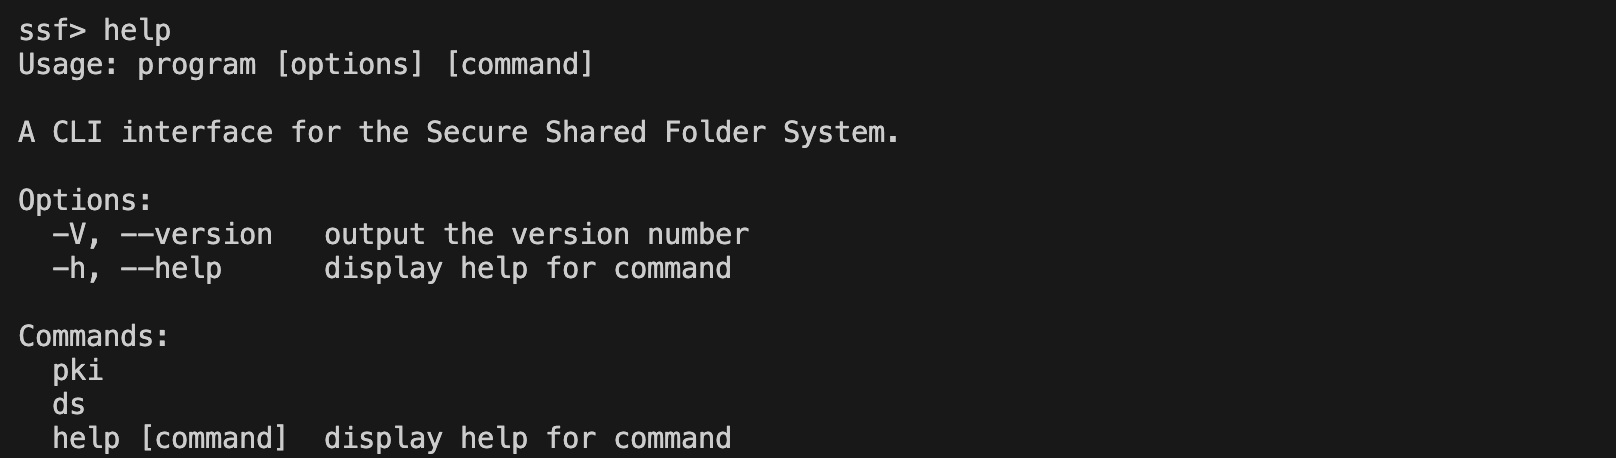
\includegraphics[width=0.8\textwidth]{figures/climain.png}
    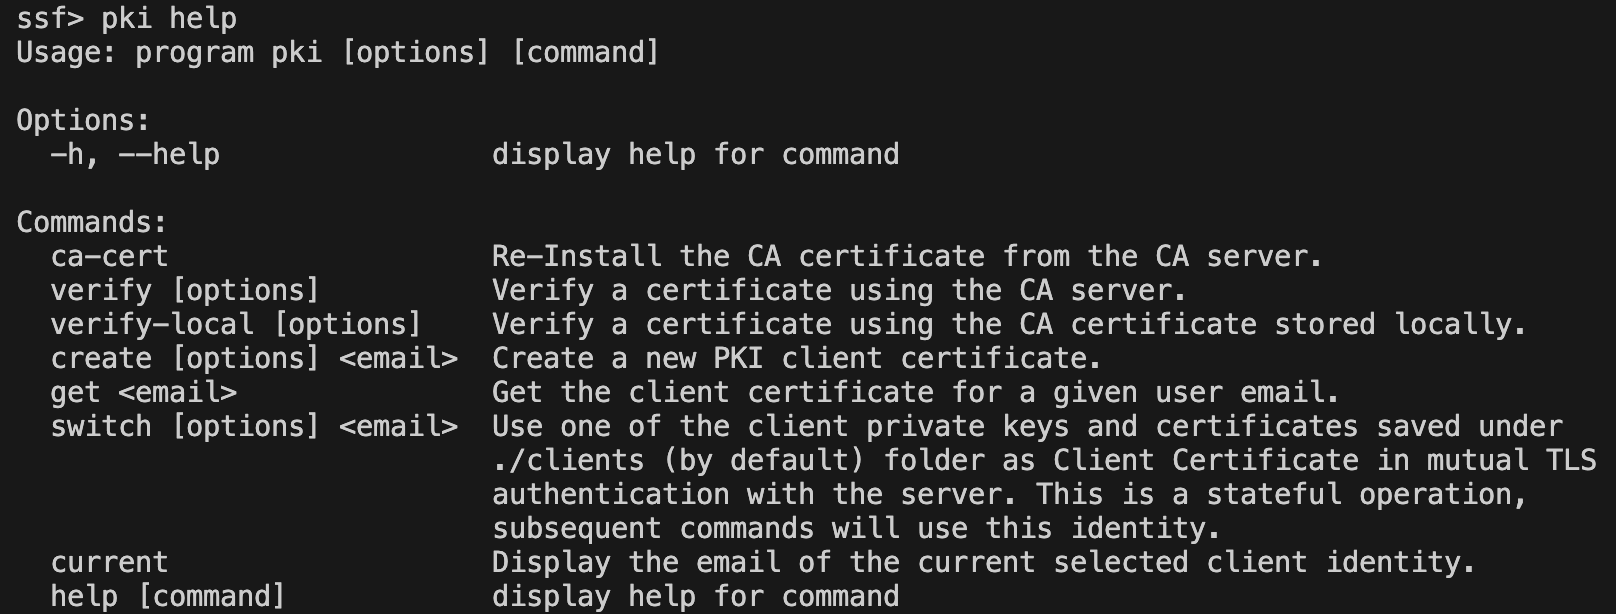
\includegraphics[width=0.8\textwidth]{figures/pkimain.png}
    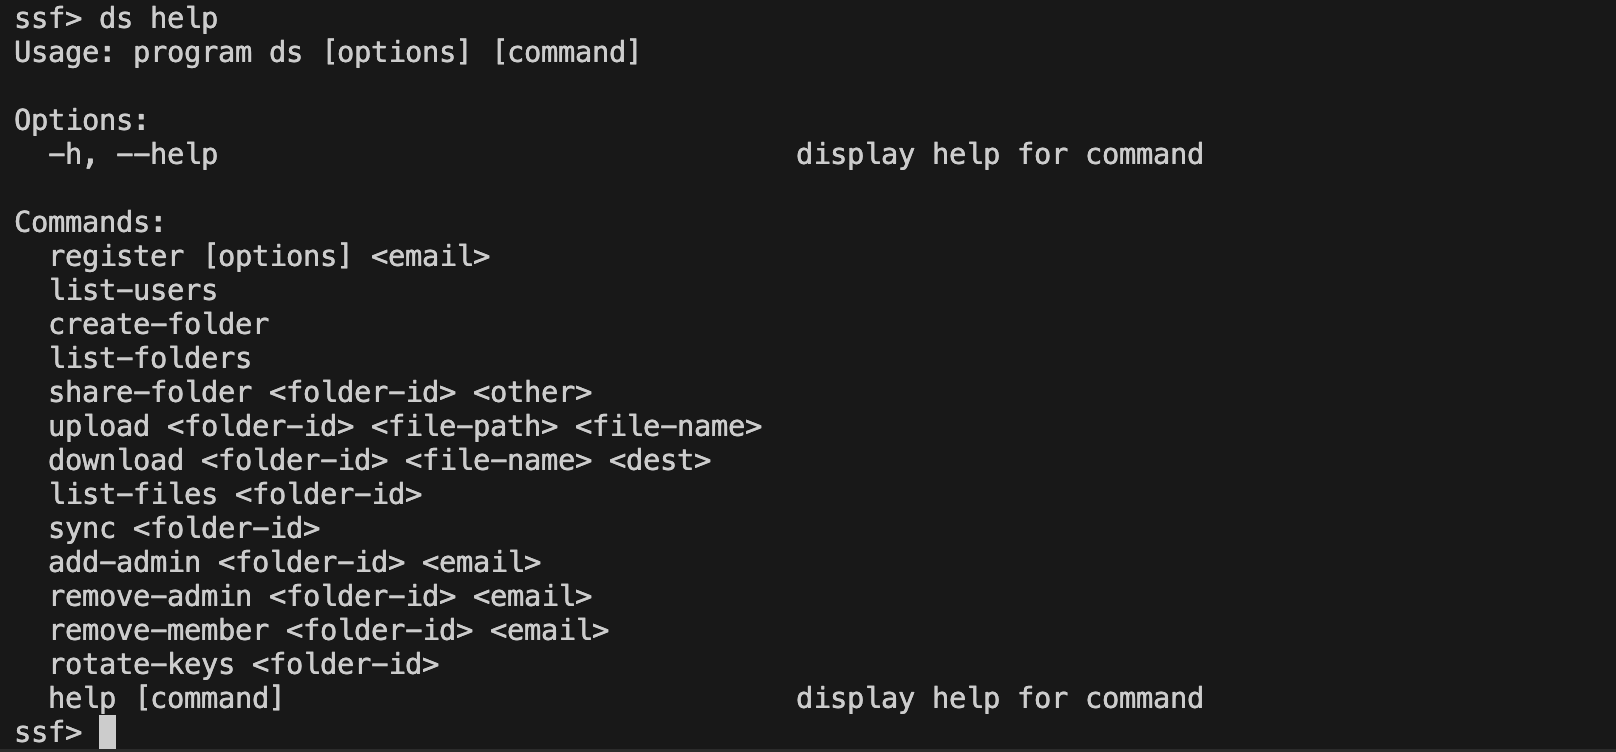
\includegraphics[width=0.8\textwidth]{figures/dsmain.png}
    \caption{CLI commands}
    \label{fig:climain}
\end{figure}

We remind the reader that some advanced functionalities
are not implemented in the baseline, therefore  
admin related commands from the ``ds'' subcommand group
return an error if the baseline protocol is used.

\paragraph{Interactive Mode}
We build the CLI interactivity using
\texttt{node:repl} module from Node.js.
The user has access to a shell-like environment
which provides command history out of the box.
The CLI can be configured to use either the
baseline protocol (\cref{ch:baseline}) or the
SSF protocol (\cref{ch:ssf}) through the environment
variable \texttt{PROTOCOL}.

\paragraph{State Management}
The baseline implementation is stateless apart
from the user identity private key, which are
stored locally in the filesystem.
The SSF implementation is stateful,
as it stores locally the cryptographic state
associated with each shared folder.
Due to library limitations explained in \cref{sc:js-bindings-for-mls}, 
we are not able to entirely persist the state of the client between invocations
when running the SSF protocols. This issue will be
fixed in future releases of the client.
For now, the CLI should be used in the interactive mode,
to maintain the client state between calls.

\subsection{Web App Setup}
The folder \texttt{www} showcases the setup
of the web application. The application is not
yet implemented, but we leave it as a reference
and to show that all the cryptographic code
we import from Wasm modules can be used
in the browser environment as well.
Interested practicioners should check
the configuration files inside \texttt{www} folder.
To create the final JS of the application
we use \texttt{Webpack}, a popular JS bundler,
which also supports loading Wasm modules.

The possibility to test some parts of the
code directly in the browser simplified some
debugging tasks, 
such as finding the compatibility issues
we describe in \cref{sc:Web-Crypto-API-implementations:-non-standard-behaviours}.



\chapter{Baseline}

\section{Motivations}

\section{Protocol}

\section{Implementation}

\chapter{Secure Shared Folder}\label{ch:ssf}

In this chapter we describe in details the Secure Shared Folder (SSF) implementation.
We detail the cryptographic implementation and usages of supporting
libraries, as well as their implications in terms of runtime execution
and the challenges we encountered (\cref{sc:ssf-sskg}, \cref{sc:ssf-double-prf}, \cref{sc:DKR-implementation}, \cref{sc:GRaPPA-implementation}). 
For each of them, we provide a description of how the implementation diverges from
the paper's construction pseudocode and the reasons behind them.
While implementing these underlying primitives indeed, we also discovered 
and fixed a few major issues, which caused failures in the 
synchronization of the cryptographic state among clients.
We detail our findings in~\cref{sc:GRaPPA-bugs}.

We also discuss the SSF Gateway modifications 
(\cref{ssc:delivery-service})
together with the SSF scheme state synchronization, persistency and rollbacks
strategies (\cref{sc:state-sync-rollbacks}). In this context,
we motivate why it would be beneficial to model precisely the
interactions between clients and servers in cryptographic
primitives that are used in a distributed setting and highlight
the gap created by loose abstraction of such communication.

We briefly describe how we perform upload and encryption of files
and their metadata and key material in \cref{sc:ssf-file-encryption}.

We provide a detailed description of some issues we encountered
while using the Web Crypto API (\cref{sc:Web-Crypto-API-implementations:-non-standard-behaviours}),
and propose a change to the API specification to solve them.
In~\cref{sc:MLS-enhancements} we also
propose enhancements to the MLS library and in general we detail
what features MLS implementations should provide to better support
the implementation of new cryptographic primitives on top of
CGKA and/or MLS.

Finally, we provide our enhancement proposals to the primitives
from~\cite{GKP}, 
such that they can better model the different client entities with respect
to their cryptographic state (\cref{sc:DKR-enhancements}).

\section{SSKG implementation: TreeSSKG}\label{sc:ssf-sskg}

The DKR construction uses SSKG, which is introduced in \cref{sc:SSKG}.
However, there is no browser-compatible implementation available to the best of our knowledge.\footnote{We found a reference Go implementation~\cite{SSKGGo}, which was used as reference together with the pseudocode in~\cite{ESORICS:MarPoe14}}
We therefore re-implement the pseudocode in~\cite{ESORICS:MarPoe14} using TypeScript.
The choice of the tree-based implementation is motivated both by its efficiency
compared to the numerical construction and because it only uses common cryptographic
primitives, such as hash functions, PRGs or block ciphers, which are supported by the Web Crypto API.
More importantly for the practical use case, is the added \texttt{SuperSeek}
functionality, which is a generalisation on top of the \texttt{Seek} procedure.
While \texttt{Seek} can only calculate an output starting from the initial state, 
\texttt{SuperSeek} can start the forward derivation from an arbitrary point of the sequence.
This allows the usage of SSKG inside the GRaPPA construction,
as we can just share the state of the SSKG chains from and until
the epochs we want to give access to. 
We pay more in terms of additional bytes sent over the wire, each SSKG
state in the tree-based construction requires up to $O(log(n))$,
where $n$ is the number of elements in the sequence generated by the SSKG.

The subfolder \texttt{ssf-client/src/protocol/sskg/} of the project contains the code for the SSKG module.
The file \texttt{sskg.ts} specify the functionalities exported by an instance of the object.
The file \texttt{treeSSKg.ts} contains the implementation of the tree-based SSKG
as a TypeScript class \texttt{TreeSSKG}. The unit tests are in \texttt{test/treeSSKG.test.ts} file,
completely covering the code, with some additional randomized tests for further validation of the code.
The \texttt{TreeSSKG} class maintains the state internally in fields:
\begin{itemize}
    \item A read-only \texttt{name}, used to identify the SSKG instance and helpful in debugging.
    \item A read-only \texttt{totalNumberOfEpochs}, a positive integer representing the total number of elements derivable from this TreeSSKG instance.
    \item A mutable \texttt{stack} field, a stack data structure, i.e. a JS array, storing the internal state of the SSKG as detailed in~\cite{ESORICS:MarPoe14}. The stack is used as a more convenient and performant way of representing a pre-order traversal on the tree structure on which the SSKG is based on. Each element of the stack is a tuple of the form $[s, h]$, where $s$ is an element in the pseudo-random sequence, stored as a byte array of type \texttt{ArrayBuffer}, while $h$ is the height of the node storing $s$ in the tree.  
\end{itemize}

The implementation required the following cryptographic operations:
\begin{itemize}
    \item Generate a starting element (seed) for the SSKG.
    \item A pseudo-random function (PRF) to derive the next element in the sequence. 
\end{itemize}

This seed is generated using the Web Crypto API \texttt{subtle.generateKey} function 
to create an HMAC SHA-256 symmetric key which is then exported to raw bytes using \texttt{exportKey}.

The Web Crypto API provides the necessary cryptographic primitives
through the \texttt{subtle} object, with the functions
\texttt{generateKey} and \texttt{deriveKey},
which support HMAC and HKDF algorithms.
We recall that the Web Crypto API representation for a
key, is made through the \texttt{CryptoKey} JS object,
which is a wrapper around the actual key material.
This object contains information about the key, such as
whether the key is a symmetric or asymmetric key, in the latter
case if it is private, the algorithm for which the key is used
and whether it can be exported or not to e.g. raw bytes.
To implement the PRF, we would need to call the \texttt{deriveKey}
function passing a HKDF \texttt{CryptoKey} to derive a new key.
The new derived key would later be used to derive the next
element in the SSKG generated sequence. However,
a call to \texttt{deriveKey} cannot produce a \texttt{CryptoKey}
designated for HKDF, thus we cannot reuse the output for a new
key derivation directly. We resort to use HMAC keys,
as we notice that the HKDF internally uses HMAC.
To assure that the bits of the keys are not truncated,
we fix the hash function to SHA-256 in all cryptographic
operations that require a hash function.
So when invoking any API call where an HKDF or HMAC algorithm are involved,
we always specify that the hash function is SHA-256.
To use the HMAC key in the key derivation, we export it
though \texttt{exportKey} to raw bytes, and then import it
back to a new \texttt{CryptoKey} designated for HKDF.
In this way the generation of a SSKG seed is done through a call
to \texttt{generateKey} to create an HMAC key, which is exported
and stored as raw bytes inside the stack data structure in the
\texttt{TreeSSKG} instance field. The PRF is then operating on the
raw bytes as explained above. The method \texttt{GetKey}
is used to retrieve a \texttt{CryptoKey} designed for HKDF.
This is done by first applying the PRF, with a \texttt{key}
label, and then importing the bytes obtained from the PRF
through \texttt{importKey}. 

In our implementation we also expose two additional methods:
\texttt{getRawKey} and \texttt{clone} which are not present 
in the SSKG primitive. 
\texttt{getRawKey} method is equal to \texttt{GetKey}
but does not perform the final import of the key, thus it 
returns the current element of the sequence as raw bytes
in an \texttt{ArrayBuffer}. 
This utility will be used in~\cref{sc:ssf-double-prf}.
The \texttt{clone} method, as the name intuitively suggests, 
is used to create a new instance
of the \texttt{TreeSSKG} class with a deep copy of the state.
\footnote{In object-oriented programming, when copying an object we normally distinguish between shallow and deep copy. 
A shallow copy is a copy of the object where the fields are 
copied by reference, while a deep copy is a copy where the 
fields are copied by value. 
In our case, we will need a deep copy of the state, 
as the state is mutable, and we want to avoid side effects 
when manipulating the copy, for example, to keep access to the current element before seeking the instance.} 
Refer to \cref{sc:DKR-implementation} for its usages inside DKR. 
Also, it has extensively been used in our unit tests, to check the equivalence
of state updates performed through the different SSKG operations.

\paragraph{Serialization} The code provides also utilities for serializing and deserializing 
the object to persist the state in the client's browser storage
as well as sending it to the other members in the group.
Since the internal state contains raw bytes, we use the concise binary 
object representation (CBOR)~\cite{rfc8949} standard to encode it. 
CBOR supports natively the encoding of byte arrays, which is not the case
for JSON.

\subsection{Asynchronous classes initialization in TypeScript}\label{pg:async-classes-init}
We highlight that all the code using the Web Crypto API is 
asynchronous by design to avoid blocking
the main thread of the browser. Blocking the JS main thread
would result in a really poor user experience, as the browser
would be unresponsive while waiting for the cryptographic
operations to complete. This introduces some complexity
when writing stateful classes like \texttt{TreeSSKG},
or later the implementations of DKR (\cref{sc:DKR-implementation})
and GRaPPA (\cref{sc:GRaPPA-implementation}), as the state
of the object is not immediately available after the constructor
is invoked. In TypeScript, one way of elegantly handling
asynchronous constructors, which are not supported, is to make the constructor private
and instance fields that require asynchronous initialization
private. Then expose a static ``factory'' method to create an 
instance of the class.
This method will return a \texttt{Promise} containing the object.
The \texttt{Promise} will be resolved after:
\begin{enumerate}
    \item The constructor has 
    completed its execution, where all synchronous available state
    is initialized, and an instance of the object has been allocated,
    but the fields requiring asynchronous initialization are still
    empty.
    \item The remaining empty private fields are also filled with the missing asynchronous state.
\end{enumerate}
Keeping the constructor private avoids any client code to
instantiate the object directly, thus protecting from
partial object state creation.
We use this pattern in all TypeScript classes that require asynchronous initialization.

\section{Sign using HMAC as a double-PRF}\label{sc:ssf-double-prf}
In \cref{sc:DPRF} we recall the notion of double-PRF security.
As we have seen, under the assumption of fixed key length HMAC 
can be used to instantiate a double-PRF secure construction.
In GRaPPA the generation of shared keys is delegated to the
DKR construction (\cref{sc:DKR-implementation}), which 
internally combines elements of fixed
length from two chains to derive a key (\cref{sc:DKR}).
In our implementation elements generated from any \texttt{TreeSSKG}
always have fixed length of 256 bits, so we can use HMAC to 
combine backward and forward chain elements together to
produce a DKR key, which will be returned by GRaPPA through
the \texttt{GetKey} operation.

The code can be found in {\texttt{ssf-client/src/protocol/doubleprf/}}.
The implementation simply accepts two byte arrays $k_1$ and $k_2$ 
as \texttt{ArrayBuffer} in input and execute the {\texttt{subtle.sign}} 
function of the Web Crypto API. 
Unfortunately again, the Web Crypto API does not provide a direct way to
use HMAC as a function that works on raw bytes. We instead
need to first import $k_1$ in a \texttt{CryptoKey} object
designated for HMAC (using SHA-256 algorithm) and sign, 
and then perform the signature
algorithm treating $k_2$ as the message to sign.
The resulting \texttt{ArrayBuffer} containing the
256 bits signature is then imported back as
a \texttt{CryptoKey} object, designated for HKDF.
We checked the underlying implementations of the Web Crypto API
both for Chrome and Node.js and made sure the bits
from both $k_1$ and $k_2$ are fully used. We remind the
reader that we have fixed our
hashing algorithm to SHA-256 in all cryptographic
objects that require a hash function. Thus, we do not provide
crypto agility, but greatly simplify and speed up the 
implementation, and have the re-assurance that the bits
of our secrets are never truncated during key derivations
because of errors with mixing different hash functions
operating on different bit vector lengths. 
We have defined global constants to specify the parameters
for the cryptographic operations in a common place,
the \texttt{ssf-client/src/protocol/commonCrypto.ts} file.

\section{DKR implementation: KaPPA}\label{sc:DKR-implementation}

In \texttt{ssf-client/src/protocol/key-progression/} we provide
the implementation and tests for the DKR primitive instantiation
D[F, S]~\cite{GKP}. In \texttt{dkr.ts} we provide the 
type definitions for a double key regression, resembling
the DKR syntax. As specified in the D[F, S] construction, we use
SSKG (\cref{sc:ssf-sskg}) to implement efficiently hash-chains supporting seek capabilities from any element of the sequence. 
We only use the methods exported by the
\texttt{SSKG} interface to implement the operations from the primitive. 
In \texttt{dkr.ts} we also provide the types for the various
concepts used in the DKR primitive (\cref{sc:background-generalised-DKR}):
\begin{itemize}
    \item An epoch is just a plain \texttt{number}, aliased as \texttt{Epoch} for readability. We recall that JS numbers are always 64-bits double precision floating point (\cref{sc:webcrypto-api}), however epochs are always positive integers (see \cref{sc:gap-type-safety-of-opaque-byte-arrays}).
    \footnote{For the curious practitioner: the TypeScript type-system allows the usage of union types, e.g. ``\texttt{type positiveUntil3} $ = 1 | 2 | 3; $''. However, the type checker in the TS compiler has an upper limit in the number of elements in a union type. Through meta programming we could generate a type to express a range of positive integers up to a given number. Again however, the TS compiler limits the recursion depth to 999 (in the version used in this project). Another option would be to write a conditional type that checks if the string representation of the number contains a dot and/or a minus sign, and returns a type \texttt{never} in these cases, the number literal otherwise. The problem with each of the options presented is that in practical terms either we hit a compiler limit or create a type which becomes unusable in practice.}
    \item An epoch interval $[l, r]$ is represented as a JS object with properties \texttt{left} and \texttt{right}, where both properties are of type \texttt{Epoch}.
    \item The DKR blocks are expressed as an enum type \texttt{BlockType}.
    \item Each forward chain is represented as a tuple of two elements $[e, ssgk]$ called \texttt{ForwardChain}, where $sskg$ is an \texttt{SSKG} object (\cref{sc:ssf-sskg}) and $e$ is the DKR \texttt{Epoch} at which we released the first element of $sskg$.
    \item Each backward chain is a tuple of three elements $[e, sskg, N]$ called \texttt{BackwardChain}, where $sskg$ is an \texttt{SSKG} object (\cref{sc:ssf-sskg}) and $e$ is the DKR \texttt{Epoch} at which we release the first element (in backward, i.e., reverse, order) of $sskg$, similarly to the forward chains, while the number $N$ specify an upper limit on the number of elements that can be generated by $sskg$. Recall that $sskg$ maintains internally a read-only property \texttt{totalNumberOfEpochs}. It follows that $N \leq$ \texttt{totalNumberOfEpochs}.
    \item We also provide a type to model an ``interval state'', which we call \texttt{DoubleChainsInterval}. An interval state is a slice extraced from a full DKR state, which gives access to forward and backward elements in a given \texttt{EpochInterval}. The property \texttt{forwardChainsInterval} (resp. \texttt{backwardChainsInterval}) contain the slices (as JS arrays) of the forward (resp. backward) chains, where the first (resp. last) chain are shrunk (\cref{sc:DKR}). We notice that both intervals and extensions of the DKR syntax map to this type.
\end{itemize}
The class \texttt{KaPPA} in {\texttt{kappa.ts}} implements the
D[F, S] construction. The state comprises:
\begin{itemize}
    \item \texttt{maxEpoch}, of type \texttt{Epoch}, representing the current epoch of the DKR state. This means for all epochs from 0 to \texttt{maxEpoch} we can get a key.
    \item \texttt{forwardChains}, a JS array of \texttt{ForwardChain}.
    \item \texttt{backwardChains}, a JS array of \texttt{BackwardChain}.
    \item A read-only \texttt{maximumIntervalLengthWithoutBlocks}, a positive integer representing the maximum number of elements that can be generated by an SSKG used internally.
    Indeed, when creating a \texttt{TreeSSKG} instance, we set the \texttt{totalNumberOfEpochs} to this value (\cref{sc:ssf-sskg}).
\end{itemize}

As recalled above, numbers are 64-bits double precision floating point in JS,
therefore the maximum epoch to which we can progress in a DKR instance is $2^{53} - 1$.
If we progress the DKR state every second, thus creating a new key
every second, this would correspond to keys for
a time span of more than 285 million years. 
Therefore, we can safely
assume that the epoch space is large enough for any practical use case.
Further we highlight that all calls to the Web Crypto API are embedded 
inside the \texttt{TreeSSKG} instances that made up the chains in \texttt{KaPPA}. 

We briefly recall that the operations of the DKR primitive are:
Init, Progress, GetInt, CreateExt, ProcExt, GetKey. Further we recall
that the operation GetKey is defined for both a full DKR state and
an interval state.
While the mathematical
description of D[F, S] does only partially distinguish between
a full DKR state and an interval state, we have chosen to model
this distinction more clearly in the implementation.
Precisely, we map an instance of \texttt{KaPPA} to a user with
read/write access to the DKR state, while a read-only
user will never construct a \texttt{KaPPA} instance, but will
only maintain and query interval states of type
\texttt{DoubleChainsInterval}. Even if the distinction does not
provide any additional cryptographic guarantee, it serves the purpose of
making the code better understandable and usable, as well
as helps in the identification of potential bugs in the implementation
or errors and enhancements in the primitives as explored in \cref{sc:correcting-primitives}.

The distinction is reflected on how the operations are attached
to the \texttt{KaPPA} class. All operations that either require
to access the full DKR state or to update it, are instance
methods of the \texttt{KaPPA} class. We call these admin methods,
as they will be used only by admins of the folders in GRaPPA (\cref{sc:GRaPPA-implementation}).
The only exception is the Init operation, which is a static method 
of the class for the motivations explained in \cref{pg:async-classes-init}.
Therefore, \texttt{Progress}, \texttt{GetInt} and \texttt{CreateExt} are all instance methods.
Diverging from the DKR syntax, they do not take the DKR state in input
as parameter, as we can access private instance state directly,
better modelling the fact that DKR is stateful.
Further, \texttt{Progress} does not return the modified state as output, 
but instead it modifies the state of the \texttt{KaPPA} instance in memory.
Modelling the primitive as a class with private state, also
allows us to easily keep multiple different instances
in memory, which is practically useful for multi-tenancy, i.e., 
for a client handling multiple shared folders with GRaPPA.
The ProcExt and GetKey operations are instead static methods,
thus usable without constructing a \texttt{KaPPA} instance,
and are the only methods that can be used by members in GRaPPA,
which do not have write access to the DKR state (\cref{sc:CGKA-implementations}).
GetKey is also defined as an instance method for convenience,
but internally it will first construct an interval state and
then call the static GetKey method on it, as described in the
DKR syntax.

We highlight that each time we need to seek a \texttt{TreeSSKG}
instance stored inside \texttt{KaPPA} forward or backward chains,
outside the \texttt{Progress} method, which is the only method
that modifies the internal state, we always clone the \texttt{TreeSSKG}
instance. This is needed to avoid side effects
deriving from the mutable state of the \texttt{TreeSSKG} instances
\cref{sc:ssf-sskg}. 

\paragraph{Serialization} As seen in SSKG, our implementation also provides utilities
to serialize and deserialize the state of the DKR object
using CBOR encoding, as we will ultimately need to
store the state in the client storage.
The upper bound on the cost of serializing the state is determined
by the number of chains (\texttt{TreeSSKG} instances),
as we need to recursively serialize the state of SSKG first.
Since we need to support also member state serialization and deserialization,
we provide static methods to serialize and deserialize interval
states of type \texttt{DoubleChainsInterval}.

\paragraph{KaPPA time efficiency}

Regarding the internals and efficiency of the D[F, S] construct
implementation \texttt{KaPPA}, we translated the helper functions 
GetFChains and GetBChains to get
slices of forward and backward chains into a modified binary search,
to avoid the linear search in the original pseudocode.
We notice that the chains are stored ordered by epoch of instantiation,
and recalling the types \texttt{ForwardChain} and \texttt{BackwardChain},
we can see that the first element of the tuples is the epoch.
We therefore have written a generic binary search function that,
given an epoch, returns the index in the array of the forward (resp. backward)
chains of type \texttt{ForwardChain} (resp. \texttt{BackwardChain})
where the first tuple element is equal to the input epoch. If the epoch is not
present, the function returns the index of the element with the 
closest epoch that is smaller than the input epoch.
As all \texttt{KaPPA} instance methods, i.e., admin operations,
are relying on these helper functions, each of them has a time
complexity of $O(log(n))$, where $n$ is the number of forward (resp. backward)
chains in the \texttt{KaPPA} instance.

\section{Using the MLS Library from JS Runtime}\label{sc:js-bindings-for-mls}

To build the GRaPPA protocol, we need a browser compatible implementation
of MLS (\cref{scc:clients}).
In this section we detail how we use and export the functionalities from mls-rs
into JS. We also give an overview of the internal state management
that is relevant for later discussions on state synchronization and resiliency
against errors (\cref{sc:state-sync-rollbacks}).
We recall from \cref{ch:setup} that mls-rs is a Rust library, which we
compile to Wasm to execute in the browser.
Further we recall that Wasm runtime has a separate memory and runs in parallel
to the JS main thread in a separate execution environment, however, communication
is possible across boundaries. Some restrictions apply to the data types
that can be transferred between the two environments, as Wasm natively supports
only numeric types and arrays. Thus, the general strategy 
is to minimize sending objects or any other complex data structures 
while writing our bindings.

\paragraph{Compilation and Dependency Management}
As we are using \texttt{wasm-pack} to compile mls-rs to Wasm, we automatically
get a ready to use JS module, including the type definitions for TypeScript,
which can be installed as a NPM dependency. The \texttt{wasm-pack} also 
provides the JS shim to allow sending strings and work with the Wasm linear
memory. Further, we can compile asynchronous Rust code to Wasm, as support is also
provided by the toolchain. For details, see the documentation in~\cite{WasmBindgen}

The code for exposing the mls-rs functionalities is provided in the Rust library crate
\texttt{ssf/}. We detail how to compile the code in the \texttt{README.md}
as well as how to run the unit tests written with \texttt{wasm-bindgen-test}.
We remind the reader, that the tests successfully execute both in Chrome browser and Node.js.
The crates from AWS mls-rs library are included in \texttt{Cargo.toml}
file, where we specify our own branch of the repository which 
includes the changes we made to the library to fix the compatibility issues
with Node.js (\cref{sc:MLS-enhancements}). From the library, we use the following crates:
\begin{itemize}
    \item \texttt{mls-rs}: the main library for the MLS protocol, exporting the Rust client and state storage in-memory providers.
    \item \texttt{mls-rs-crypto-webcrypto}: the cryptographic provider implementation for Wasm target. This is based on the Web Crypto API.
    \item We further explicitly specify the \texttt{mls-rs-core} crate, because we want to use our own branch of the library and enable the compilation options needed for the compatibility.
\end{itemize}

For practicioners, although missing from the library documentation, we highlight that
the correct compilation of the library to Wasm is possible only by enabling the
compiler flag \texttt{rustflags = "--cfg mls\_build\_async"}. This option is added
to the \texttt{Cargo.toml} under the \texttt{[build]} stanza.

\paragraph{Error Handling}
The mls-rs library uses an internal error type to handle errors, as generally
done in Rust. The \texttt{MlsError} enum represent all the possible errors generated
by the library, with their description.
In the JS bindings written in \texttt{ssf/lib.rs} every function returns a Rust
\texttt{Result} type, expressing either a successful result or an error.
The error is always converted to a string, the description of the error itself,
before sending it to JS. 
Note that since all the functions we export are asynchronous,
the \texttt{Result} is converted to a JS \texttt{Promise} in the JS shim.
A \texttt{Promise} object in JS represents the eventual completion (or failure) 
of an asynchronous operation, and its resulting value or error.
When calling the bindings from our TypeScript client implementation,
we can therefore easily handle the errors,
as if the code was natively written in JS.

\paragraph{Application Messages}
The main entry point of the library is the \texttt{Client} struct, which
is an object providing functionalities to create a MLS (internally CGKA)
group and evolve its state. Further, the \texttt{Client} allows the creation
and encryption of application messages (\cref{sc:MLS}). While in the pseudocode 
of GRaPPA there is no explicit mention to MLS protocol, but only to CGKA,
we notice that while executing the operations of the GRaPPA protocol,
parts of the control message are encrypted through advanced authenticated
encryption standard (AEAD) using the CGKA shared epoch secret.
Instead of manually implementing this encryption, we just use the
support for application messages provided by MLS. This difference highlights
that although for demonstration purposes the MLS protocol is kept out of scope,
practically the GRaPPA protocol is build on top of MLS and not only CGKA, 
and further motivate our choice to use an MLS library.

\paragraph{Key Packages}
The \texttt{Client} object provides also functionalities to create
key packages, which are the cryptographic material needed to invite
a new member to the group. A key package can be created through the provided
bindings and returned as a \texttt{Uint8Array}, the serialization and
deserialization of the key package (when processing it) is handled by the 
library itself. 


\paragraph{State Management}
A \texttt{Client} object can handle multiple MLS groups.
An abstraction layer on top of the storage is provided by the library,
thus allowing for different storage providers to be implemented and used.
The core library provides an in-memory storage provider.
The \texttt{mls-rs-provider-sqlite} crate implements a storage provider
on top of the relational database engine SQLite. However, this is not compatible
with the Wasm target, as SQLite is not available in the browser environment.

We resort on the in-memory storage provider, which is not persisted
across browser sessions. We propose an implementation of a browser compatible
storage provider in~\cref{sc:MLS-enhancements}, but leave it out of scope
for this project, because of the time constraints.
A further problem arising when using the in-memory storage provider
is that since we are making calls from the JS runtime to the Wasm runtime,
after a call to the Wasm runtime ends, the Wasm memory would be freed and
therefore the state would be lost.
We solve this problem by instantiating the storage provider related objects
in a lazy-initialised global map addressed by used identity, which is kept in
the Wasm memory across calls. This hack is not ideal and only temporary,
until we implement a browser compatible persistency solution.
Also, to avoid losing the changes in the group state between calls to
exported functions, we need to write the state back to the storage provider
after each operation that modifies it.

On a related note, we recall that the MLS protocol is using a proposal
and commit mechanism to evolve the state of the group (\cref{sc:MLS}).
The \texttt{Client} object can be used to get a handle to the \texttt{Group}
object, which is the main interface to interact with a CGKA group.
The \texttt{Group} object provides functionalities to create proposals,
commit them, and apply the state changes. Further, it also provides
functionalities to encrypt and decrypt application messages.
We notice that creating a commit message, which is the final step
in the proposal and commit mechanism, does not update the \texttt{Group}
current state until a call to apply the changes is made on the object.
In between the creation of the commit message and the
application of the changes, the \texttt{Group} object maintains
the pending commit in a staging area~\cite{AWSMLSGroup}.
This staging area is also persisted in the storage provider.
However, the modifications to the cryptographic state of the group
deriving from the pending commit are not taken into consideration
when encrypting application messages, i.e., the encryption
is done using the current state of the group only, and not the pending commit.
This limitation has effects on the state synchronization and rollbacks
as described in \cref{sc:state-sync-rollbacks}.


\section{Delivery Service}\label{ssc:delivery-service}

The delivery service (DS) is a new component of our system needed 
to support the usage of MLS (\cref{sc:MLS}).
The DS is responsible for delivering messages to clients in order.

We implement the abstract functionalities of the DS inside our server existing SSF Proxy
server. As the SSF Proxy server is already responsible for the creation of folders,
authentication of users, and the access control of users to folder, 
it is a natural choice to extend its functionalities to also provide APIs
for the DS.
To this end we modify and extend the SSF Proxy server and its SQL database as described
in the following of this section.
In short, we add new endpoints to receive, fetch and acknowledge
GRaPPA control messages, as well as key packages.
We store in the ``ds'' MySQL database the new entities, and use the
DB transaction support to synchronize multiple clients executing
the GRaPPA protocol. Further we use the server as a broadcaster to
deliver the messages to the clients in order. The ordering guarantee
is provided by our usage of MySQL.

\paragraph{Additional Database Entities}
We extend the SQL database ``ds'' with three different tables:
\begin{itemize}
    \item \texttt{key\_packages} storing the key packages (\cref{sc:js-bindings-for-mls}) generated by the MLS clients for later retrieval by a different user which wants to send an invitation to join a folder.
    \item \texttt{pending\_group\_messages} storing the first part of a GRaPPA control messages of type \texttt{Proposal} that are pending and need to be delivered to the clients (\cref{sc:GRaPPA-implementation}).
    \item \texttt{application\_messages} storing the second part of a GRaPPA control messages of type \texttt{ApplicationMessageForPendingProposals}, that are pending and needs to be delivered to the clients (\cref{sc:GRaPPA-implementation}).
\end{itemize}

All the data from the client is sent as a byte array, and stored in each table
directly by the server. The server is not aware of the content of the messages,
and does not need to be.

The \texttt{key\_packages} table has the following columns:
\begin{itemize}
    \item \texttt{key\_package\_id} as a primary key, a unique autoincremented identifier for the key package.
    \item \texttt{key\_package} as a \texttt{BLOB}, storing the key package.
    \item \texttt{user\_email} a foreign key to \texttt{users.user\_email}, storing the email of the user that created the key package. A \texttt{CASCADE DELETE} constraint is set to delete the key package when the referenced user entity is deleted to automatically clean up the database.
\end{itemize}
Key packages do not belong to a folder, but just to a user, and are used to
add a new user to a folder in GRaPPA, since the user needs to be added to the
member CGKA group (\cref{sc:gkp-scheme}).

The \texttt{pending\_group\_messages} table has the following columns:
\begin{itemize}
    \item \texttt{message\_id} as a primary key, a unique \texttt{INTEGER} autoincremented for the message.
    \item \texttt{payload} as a \texttt{BLOB}, storing the message.
    \item \texttt{folder\_id} a foreign key to \texttt{folders.folder\_id}, storing the unique identifier of the folder to which the message belongs. A \texttt{CASCADE DELETE} constraint is set to delete the message when the referenced folder entity is deleted to automatically clean up the database.
    \item \texttt{user\_email} a foreign key to \texttt{users.user\_email}, storing the email of the user to which the message has to be delivered. A \texttt{CASCADE DELETE} constraint is set to delete the message when the referenced user entity is deleted to automatically clean up the database.
\end{itemize}
We point out that since we store messages by \texttt{user\_email} we are replicating
the \texttt{payload} content for each user that is part of the folder 
referenced by \texttt{folder\_id}. This will be changed and was done as a first
development iteration to simplify the implementation. Ideally this table should be
normalized, and a new table containing only the \texttt{message\_id}
and the \texttt{payload} should be created, to store the content of the messages
indipendently from the receiving users.

This table is effectively modelling an ordered queue of messages:
the messages are globally ordered by insertion time through the \texttt{message\_id},
so for each user and folder, the subset of messages belonging to that
user and folder is also ordered by insertion time.
We call a queue the ordered subset of messages belonging to a user and folder in the table.
We will see in the API description how the server guarantees consistent state updates
of the clients.

The \texttt{application\_messages} table has the following columns:
\begin{itemize}
    \item \texttt{id} as a primary key, a unique \texttt{INTEGER} autoincremented for the application message.
    \item \texttt{message\_id} a foreign key to \texttt{pending\_group\_messages.message\_id}, storing the unique identifier of the message which is completed by this application message. A \texttt{CASCADE DELETE} constraint is set to delete the application message when the referenced pending group message entity is deleted to automatically clean up the database.
    \item \texttt{payload} as a \texttt{BLOB}, storing the message.
\end{itemize}

This table stores the second part of the GRaPPA control messages, which reference 
the first part stored in the \texttt{pending\_group\_messages} table.
Similarly, we simplify and speed up development by replicating the
payload for each foreign key to a pending group message.

\paragraph{DS APIs}
We extend the SSF Proxy server with the following new endpoints to support the DS functionalities:
\begin{itemize}
    \item \texttt{POST /users/keys}: upload a key package.
    \item \texttt{GET /users/<folder\_id>/keys}: fetch and delete a key package given an existing folder id. The folder id parameter is needed for access control, to verify that the user requesting the key package of another user is part of the corresponding folder. The server will return an error in case the user for which the key is requested is already part of the given folder.
    \item \texttt{POST /folders/<folder\_id>/proposals}: upload the first part of a GRaPPA control message for the specified folder. The server checks that the sender identity is part of the folder is part of the folder, and that the user's pending message queue for the folder is empty. The upload will transactionally check and update the database, inserting the message in the \texttt{pending\_group\_messages} table, replicated for each user in the folder as known by the server through the \texttt{users\_folders} table, excluding the sender user.
    \item \texttt{PATCH /folders/<folder\_id>/proposals}: upload the second part of a GRaPPA control message for the specified folder and message ids sent in the request body. The server performs the usual access control checks, and transactionally check and insert the message in the \texttt{application\_messages} table, replicated for each message id in the request body. This a PATCH request, as logically it is patching the first part of the GRaPPA control message with the second part. Furthermore, a notification containing the folder id is sent to the clients receiving the message, to signal that they need to try fetching new GRaPPA control messages from the server. 
    \item \texttt{GET /folders/<folder\_id>/proposals}: fetch the first GRaPPA complete control message for the specified folder from the user's queue. The server checks that the user is part of the folder, and returns the first pending message together with the corresponding application message if available.
    \item \texttt{DELETE /folders/<folder\_id>/proposals/<message\_id>}: delete the GRaPPA complete control message for the specified folder and sender user. The server deletes both related entries, transactionally from the tables \texttt{pending\_group\_messages} and \texttt{application\_messages}.
    \item \texttt{PATCH /v2/folders/<folder\_id>}: given the folder id, share the corresponding folder with the user specified in the request body. The body further includes the bytes of the first part of the GRaPPA control message which invites the new member to the folder. Since this operation requires a different DB transaction to be performed compared to the original version of the endpoint, we defined a v2 version of the endpoint to also avoid regressions in the baseline implementation.
\end{itemize}

We notice that, although in the GKP scheme and in the GRaPPA construction nor capture the
interaction with the server, neither the server
is assumed to hold any state, in our implementation we
need to take both things into account. 
The DS state, which is made up by the pending messages, reflects the fact that
the cryptographic state of the clients for which the queues are non-empty,
is out of sync with respect of other group members.
We will discuss the implications in \cref{ssc:GKP-client-middleware} and \cref{sc:state-sync-rollbacks}.

\section{GKP Implementation}\label{sc:GRaPPA-implementation}

The group key progression (GKP) primitive (\cref{sc:SSF}) is instantiated in the
GRaPPA construction, of which the pseudocode is provided in~\cite{GKP}.
We implement GRaPPA in TypeScript, similarly to the DKR primitive.
The code can be found in \texttt{ssf-client/src/protocol/group-key-progression/},
including the unit tests in \texttt{test/grappa.test.ts}.

\paragraph{Types Design}
As in the other primitive implementations,
we provide the TS types for the GKP entities used 
in the GRaPPA construction (\cref{sc:gkp-scheme}) inside the \texttt{gkp.ts} file:
\begin{itemize}
    \item We model the state of both members and admins as TS interfaces. 
    TS interfaces are extendable, so we factor out the common
    properties to keep our code DRY in the type definitions.\footnote{DRY stands for Don't Repeat Yourself, a software development principle that aims to reduce repetition of code patterns.}
    Having shared properties factored out also make them always
    available to the type checker while writing common code paths for both members and admins.
    In the \texttt{BaseState}, the \texttt{cgkaMemberGroupId} property stores the unique identifier of the group to which all members belong to. We will use the unique folder id returned by the SSF Proxy server at folder creation (\cref{sc:ssf-proxy-server}). This is represented as an opaque \texttt{Uint8Array}. 
    The interface \texttt{MemberState} extending the \texttt{BaseState} adds:
    \begin{itemize}
        \item A \texttt{role} property, a literal string \texttt{member}.
        \item An \texttt{interval} property, of type \texttt{DoubleChainsInterval}, storing the interval state to which the member has been given access to (\cref{sc:DKR-implementation}).
    \end{itemize}
    The admin state modelled in \texttt{AdminState}, also extending \texttt{BaseState}, adds:
    \begin{itemize}
        \item A \texttt{role} property, a literal string \texttt{admin}.
        \item A \texttt{cgkaAdminGroupId} property, of type \texttt{Uint8Array}, storing the unique identifier of the group to which all admins belong to. We will deterministically construct this identifier concatenating a prefix \texttt{ADMIN-} with the \texttt{cgkaMemberGroupId} 
        \item A \texttt{dkr} property, holding an instance of \texttt{KaPPA} (\cref{sc:DKR-implementation}).
    \end{itemize}
    Finally, a type \texttt{ClientState} represents either a member or an admin state, and will be used
    inside the \texttt{GRaPPA} class.
    \footnote{As the \texttt{MemberState} and \texttt{AdminState} interfaces 
    extend the \texttt{BaseState} interface and they both declare 
    a \texttt{role} property, after a check for the value of role in the code,
    the compiler will be able to infer which properties are available in the object, 
    providing type safety and avoiding runtime errors. This type system feature is called discriminated union.~\cite{TSDisciminatedUnions}.}
    
    \item We define the types corresponding to each command from GKP (\cref{sc:gkp-scheme}),
    and we make clear distinction between commands that target another user and commands that
    target the user executing them.\footnote{To avoid bloating the description, we forward to the code for the details. We again make use of discriminated union modelling each command with its own type.} 
    We notice that the arguments to \texttt{ExecCtrl} all take
    either zero or one argument, which is the target user identifier.
    The type \texttt{ControlCommand} is a union of all the possible types of commands.

    \item The \texttt{Proposal} type partially represent the messages exchanged in GRaPPA 
    to carry out the various commands. The name carries out the semantic
    that a proposal could be rejected by the system (\cref{sc:state-sync-rollbacks}).
    Each proposal embeds a property \texttt{cmd}
    specifying the exact type of the command and its arguments if any.
    Then, depending on the \texttt{cmd}, the proposal will additionally contain:
    \begin{itemize}
        \item \texttt{memberControlMsg}, a \texttt{Uint8Array} containing the encrypted member CGKA control message (all). Corresponds to the variable $T_M$ in the pseudocode.
        \item \texttt{memberWelcomeMsg}, a \texttt{Uint8Array} containing the CGKA welcome message for a new joining member (\texttt{Add}). Corresponds to variable $W_M$ in the pseudocode.
        \item \texttt{adminControlMsg}, a \texttt{Uint8Array} containing the encrypted admin CGKA control message (\texttt{AddAdm}, \texttt{RemAdm}, \texttt{UpdAdm}, \texttt{Rem}, \texttt{RotKeys}). Corresponds to the variable $T_A$ in the pseudocode.
        \item \texttt{adminWelcomeMsg}, a \texttt{Uint8Array} containing the CGKA welcome message for a member which is granted admin privileges (\texttt{AddAdm}). Corresponds to variable $W_A$ in the pseudocode.
    \end{itemize}

    \item The \texttt{AcceptedProposal} type is used to model a \texttt{Proposal}
    that has been accepted by the delivery service (\cref{ssc:delivery-service}),
    and is therefore considered applied in all clients state, meaning that
    the changes specified in the proposal fields, which are CGKA proposals (\cref{sc:CGKA}),
    have been committed inside the respective CGKA state (\cref{sc:js-bindings-for-mls}, \cref{sc:state-sync-rollbacks}).
    An \texttt{AcceptedProposal} is a \texttt{Proposal} with the additional \texttt{messageId} field of type \texttt{number},
    which is a unique global identifier of the message in the system, and is added by the DS if the proposal is accepted.

    \item \texttt{ApplicationMessageForPendingProposals} is the type modelling a partial message exchanged in GRaPPA
    to carry out the various commands. The name carries out the semantic of being composed of 
    MLS application messages (\cref{sc:MLS}). This message is sent to the delivery service
    with references to the \texttt{AcceptedProposal} that are completed by this application
    message, meaning that they constitute together the full control message (or welcome message) as described in
    GRaPPA~\cite{GKP}. The references are a list of \texttt{messageId}, i.e. an array of \texttt{number}.

\end{itemize}

The reader should notice the difference between the modelling of message exchange
in the GRaPPA construction and in the implementation. This
difference can be seen already in the types, where the \texttt{Proposal} type is only 
partially modelling the return values from the operations of 
GRaPPA pseudocode, representing only the CGKA control messages. 
As described in \cref{sc:js-bindings-for-mls},
the library mls-rs does not allow a stashed change in the internal 
cryptographic group secret of CGKA that has not been fully applied,
i.e. the state is advanced and there is no possibility to rollback, 
to encrypt an application message until the proposals are committed and applied. 
Thus, we need to split proposals and commits from what we call GRaPPA application messages (\cref{sc:state-sync-rollbacks}, \cref{ssc:delivery-service}).

\paragraph{Object-oriented Design}
Inside \texttt{gkp.ts}, we also provide the interface exposing the functionalities 
of the \texttt{GKP} primitive (\cref{sc:gkp-scheme}). 
The procedures \texttt{JoinCtrl} and \texttt{InitUser} are however not instance
methods of the class, but static methods. This is because one is used to create
a GRaPPA client to actively create a new group, while the other is used to
join an existing group to which we are invited. 

The TS class \texttt{GRaPPA} implements GRaPPA and maintains the state internally, similarly to the \texttt{KaPPA} class.
The class holds the following state:
\begin{itemize}
    \item \texttt{uid}: the \texttt{Uint8Array} representing the unique identifier of the user, this corresponds to the \texttt{user\_email} in the public certificate from the PKI and with which the user register itself to the SSF Proxy.
    \item \texttt{middleware}: an instance of the \texttt{GKPClientMiddleware} class, which is used to abstract away calls to the backend. It is injected in the constructor of the class, it is useful mostly for testing purposes (\cref{ssc:GKP-client-middleware}).
    \item \texttt{state}: an object of \texttt{ClientState} type, which is either a \texttt{MemberState} or an \texttt{AdminState} depending on the role of the user in the group. As this field depends on the user being part of a group, it is \texttt{undefined} until either \texttt{JoinCtrl} or \texttt{Create} are successfully executed. 
\end{itemize}

Similarly to what is happening in \texttt{KaPPA}, \texttt{GRaPPA} methods changing the state
do not return the new state, but instead apply the changes to the internal one.
Each method when executed successfully, will also try to serialize the state to persistent
storage before completing (\cref{ssc:GKP-persistent-storage}).


\subsection{GKP Client Middleware}\label{ssc:GKP-client-middleware}
One of the major differences between GRaPPA and the implementation in \texttt{GRaPPA}
is the real interaction with a server, which is interleaved in the protocol execution (\cref{sc:state-sync-rollbacks}).

We abstract away this interaction in \texttt{GKPClientMiddleware} type, also
defined in \texttt{gkp.ts}. The middleware is used to handle serialization of
\texttt{Proposal} and \texttt{ApplicationMessageForPendingProposals} objects
to byte arrays using CBOR and to send them to the server using the autogenerated
APIs from the OpenAPI specification of the SSF Proxy server (\cref{sc:ssf-proxy-server}).
This enhances readability of the \texttt{GRaPPA} code, as well as maintainability,
as the code for the communication with the server is kept in a single place.
We implement the middleware in the \texttt{dsMiddleware.ts} file.
A mock implementation is provided in the \texttt{inMemoryMiddleware.ts} file, 
and it is used to test the \texttt{GRaPPA} class in isolation from the server.
We highlight that the serialization code for the message is kept separate
from the implementation of GRaPPA, as the \texttt{GRaPPA} class should ideally only
deal with the cryptographic operations.

\subsection{GKP Persistent Storage Abstraction}\label{ssc:GKP-persistent-storage}
Another difference between the GRaPPA construction and its implementation
is the need to persist the state of the client
to ensure that a change is not lost in case of a crash
or any other event that would wipe out the volatile memory.
This, similar to database transactions, has to be done
in a precise way, to ensure the possibility of recovering a
consistent state of the client in case of errors (\cref{sc:state-sync-rollbacks}). 

As in \cref{ssc:GKP-client-middleware} we abstract away the interaction
with the persistent storage layer to keep our
\texttt{GRaPPA} class clean and focused on the cryptographic operations.
The persistency layer is implemented in the \texttt{storage.ts} file.
A TS interface \texttt{GKPStorage} together with the types expressing
the format of the serialized state. For the serialization and
deserialization we first recursively operate on each
internal complex property, like \texttt{dkr}, deferring to
the specific serialization and deserialization methods of the
respective classes. Then we serialize the state to a byte array
using CBOR. In the Node.js CLI client, we store
the serialized state in a file, while in the browser client
we would need an Indexed DB compatible implementation of the
aforementioned \texttt{GKPStorage} interface, which was left
out of scope for now.

We remind the reader, that although we are able to serialize
the state kept in the \texttt{GRaPPA} class,
the state of the MLS client running in Wasm is not persisted
in long term storage (\cref{sc:js-bindings-for-mls}).
Although this is a blocker for the deployability of the system,
we still structure the code in such a way that fixing this
issue will allow us to have a fully-functional system.

\subsection{State Synchronization and Transactions}\label{sc:state-sync-rollbacks}

Global state synchronization and state rollbacks are a crucial part of the \texttt{GRaPPA} implementation,
to maintain the consistency of the group state across all clients, which is 
key for a client own ability to continue to operate and access the folder in case of
errors or rejection of a proposal by the DS.

Ideally, the middleware calls should not be interleaved with the cryptographic operations.
We would like to have a unique GRaPPA control message, including both parts we model in our types, 
to be sent to the server
at once and then delivered to all recipients.
However, as we have seen in \cref{sc:js-bindings-for-mls},
since we are calling the mls-rs library across process boundaries, i.e. from JS
runtime into Wasm runtime, we cannot avoid writing the changes to the state
in the persistent storage.
Further, the DS, hence the SSF Proxy server, needs to ensure that messages are delivered in
a global order to all clients, and is offloaded the responsibility to 
keep the client synchronized (\cref{ssc:delivery-service}).

Let's consider the case where a client starts executing a \texttt{ExecCtrl} operation:
the client needs first to check if the operation is accepted by the DS,
and then apply the changes to the state. The only trusted source of truth
on the synchronization status of the system among clients of a folder is
the DS, as the DB is acting as a global transactionally consistent state.
Now if the client proposing a change to the group state tries to send it
to the DS, and the DS rejects the proposal, the client should roll back the changes as well.
Since there is no way to roll back the changes with the in-memory storage provider
of the mls-rs library, we therefore need to split the GRaPPA control messages
in two parts, as already explained when describing the types in \cref{sc:GRaPPA-implementation}
and the DS API in \cref{ssc:delivery-service}.
Now that we have motivated the choice, the GRaPPA \texttt{ExecCtrl} protocol is modified as follows:
\begin{enumerate}
    \item Depending on the operation, the client propose and commit the respective changes internally to the CGKA group state, some of these operation involve both member and admin CGKA groups. The pending commit(s) is written to the in-memory storage (inside Wasm).
    \item The client sends the first part of the GRaPPA control message (of type \texttt{Proposal}) to the server, through the \texttt{POST} proposal endpoint. In case the operation originating the proposal is the addition of a new member to the folder, use the v2 \texttt{PATCH} folders endpoint (\cref{ssc:delivery-service}).
    \item The DS process the \texttt{POST} proposal request (or v2 \texttt{PATCH} folders request) and answers accordingly to whether the pending message queue for the sender in the targeted folder is empty or not:
    \begin{itemize}
        \item accept the message and send back all the \texttt{messageId} created by the DB to the client;
        \item reject the message and send back an error to the client.
    \end{itemize}
    \item In case an error is received, the client discards the pending commit(s), thus rolling back the changes to the CGKA group state(s). The client will then try to sync the outdated local state, by fetching the latest GRaPPA control messages from the DS until \texttt{Not Found} error is returned, and returns an error to the user instructing to re-try the operation.
    \item If the \texttt{POST} proposal call is successful, the client applies the changes to the state. 
    \item Then it computes the application message and encrypts it through a call to the JS bindings. At this point the encryption will be performed with the updated CGKA epoch secret. 
    \item Send the second part of the GRaPPA control message to the DS. Retry with an exponential backoff in case of errors.
    \item Finalise the operation, by also serializing and persist the eventual changes to the internal \texttt{dkr} object.
\end{enumerate}

\section{SSF Implementation: File Encryption Management}\label{sc:ssf-file-encryption}


\section{Web Crypto API implementations: non-standard behaviours}\label{sc:Web-Crypto-API-implementations:-non-standard-behaviours}

In this section we describe a gap in the Web Crypto API specification and
implementation which creates a portability issue affecting the mls-rs library
and, in general, the deployability of advanced cryptographic primitives
in the browser environment.

AWS mls-rs library implementors made the library available to Wasm compilation
targets. The support is experimental, and involves for now only the implementation
of the cryptographic operations needed to execute MLS on top of the Web Crypto API.
\footnote{For practicioners: the library abstracts the underlying cryptographic code in Rust traits which are implemented for different runtime environments/cryptographic providers. The one used for the Wasm target is implemented in the crate \texttt{mls-rs-crypto-webcrypto}.}
While looking at the history commits of the library, we found out that
apparently the support for Wasm builds was added only for Chrome runtime.
Indeed, integration tests are available
which prove the compatibility and avoid regressions in Chrome.
However, as seen in \cref{ch:setup} we use Node.js to develop our client
CLI to avoid dealing with a UI in our first implementation.
Thanks to our multi-runtime setup, we discovered the portability issue
hidden in the library and in the implementations of the Web Crypto API.

When using elliptic-curve crypto primitives, the mls-rs library is 
calculating the public key from the bytes of a DER-encoded~\cite{Kaliski2002ALG} private key 
by passing the bytes of the key to the Web Crypto API \texttt{importKey}
call~\cite{WebCryptoAPIImportKey}. In Chrome, the underlying BoringSSL~\cite{BoringSSL} on which the Web Crypto API 
are implemented on, calculates
the public part of the key which is appended to the bytes provided in input.
However, this behaviour is non-standard and is not supported in other
major Web Crypto API implementations:
\begin{itemize}
    \item In Node.js, the \texttt{importKey} call will just import the key into a \texttt{CryptoKey} JS object, without any error~\cite{WebCryptoAPICryptoKey}. However, the underlying bytes are not modified. The mls-rs library has a check to detect the missing public key part and will then throw a runtime error. No documentation is provided on this issue, and we discover it by debugging the library compiled in Wasm, which is not a trivial task. In the end we resorted on reading the source code. Although the documentation states that the cryptographic support is only experimental, it would be beneficial to add more details on this problem.
    \item In Safari, the \texttt{importKey} call will throw an error.
    \item In Firefox, the \texttt{importKey} call will throw an error.
\end{itemize}

The only case we could develop a work-around for is Node.js. Since in this runtime
the public key is not calculated but at the same time the operation does not fail,
after importing the private key we can force the calculation of the public key with an additional
export/import operation to \texttt{jwk} back to \texttt{pkcs8}~\cite{JsonWebKey, rfc5958}.
Indeed, by performing this \texttt{exportKey} call to produce the \texttt{jwk}
representation of the key, the curves coordinates $x$ and $y$ are calculated.
Therefore, importing back the key in \texttt{pkcs8} format will produce the correct
public key. The code is published in a pull request to the mls-rs library~\cite{AWSNodeJSCodeContributions}.

We notice that the mls-rs uses the Web Crypto API in a way conforming to the
specification, as the definition of the DER-encoded private key does not
restrict to the usage of elliptic curves private key info which must 
contain the public key field, but only should~\cite{rfc5915}:
\begin{quote}
    publicKey contains the elliptic curve public key associated with
    the private key in question.  The format of the public key is
    specified in Section 2.2 of [RFC5480].  Though the ASN.1 indicates
    publicKey is OPTIONAL, implementations that conform to this
    document SHOULD always include the publicKey field.
\end{quote}
We further notice that mls-rs implementation use case seems legitimate,
as the public key calculation would require non-constant time code
to execute on top of a secret key. Therefore, we would propose
to change the Web Crypto API \texttt{importKey} specification to
explicitly require the public key calculation, so that all
implementations are aligned with the same behaviour. In this way,
the API would support more advanced cryptographic operations on top
of the existing support for elliptic curves cryptography, such as the ones
required while trying to compute a key pair from a symmetric private key.

\section{mls-rs: Wasm build enhancements}\label{sc:MLS-enhancements}

While working with the MLS library we found out that the Wasm target
is not fully production ready:
\begin{itemize}
    \item The library is not fully portable to all major browser (\cref{sc:Web-Crypto-API-implementations:-non-standard-behaviours}).
    \item Node.js is not supported. We add support for the compiled Wasm to run in Node.js by adding bindings to the Web Crypto API implementation from \texttt{node:crypto} module of Node.js~\cite{NodeJsWebCryptoAPI}. We adapt the existing JS inline code included in the library to be compatible with the JS module resolution mechanism and syntax of Node.js~\cite{AWSNodeJSCodeContributions}.\footnote{For practitioners: JS modules evolved during the years, Node.js is using CommonJS modules, which is the standard outside browser runtimes. These modules are also used in the npm ecosystem (the package manager for JS). The syntax of CommonJS is using plain JS objects and functions (require) to perform import and exports. Browsers use currently ES modules, which were added in 2015 to the JS standard and widely adopted in 2020. ES modules use the \texttt{import} and \texttt{export} keywords to perform the same operations.}
    \item The client state is not persisted and only kept in memory for now. We propose a strategy to persist the client-side state in the browser's using the Indexed Database API~\cite{MlsRsWebStorageProvider, IndexedDBAPI}.
    \item The X.509 certificates are not supported to manage identities of the users. This imposes the usage of Basic Credentials, which lower the security of the implementation as those credentials are not validated while performing group operations. We propose to add support for X.509 certificates in the library~\cite{MlsRsX509Certificates}. Our proposal aims to support the use case where the CA certificate is embedded in the client code or where the CA certificate is loaded at runtime through a different mechanism. This use case could be applied for example in a corporate environment.
\end{itemize}

\nd{propose enhancement to the library to allow encryption under stashed commits.}

\section{Correcting the primitives}\label{sc:correcting-primitives}

During the implementation and testing the GRaPPA constructions,
we found issues in the pseudocode descriptions as provided
in the original manuscript of \cite{GKP}.
In \cref{sc:GRaPPA-bugs} we provide the full explanations of the bugs, 
and the corrections we applied. 
We also discuss the implications of our corrections. 

The bugs we highlight in the following sections
derive from the underlying primitive not being expressive and
precise enough to model the interactions between distributed clients
playing either the role of admin or member.
In the generalized DKR primitive, the read/write (admin) 
and read-only (member) capabilities (see \cref{sc:DKR-implementation})
are not modelled at all in the mathematical definitions of the operations.
We explore the implications and attempt to correct
the primitive in~\cref{sc:DKR-enhancements}.

\subsection{GRaPPA bugs}\label{sc:GRaPPA-bugs}

While implementing the GRaPPA construction, we found out two bugs.
The bugs are both leading to the same issue: the state of the
sender admin and receiving admins can go out of sync after a certain
sequence of operations are executed.

\paragraph{Bug 1:} The admin operations \texttt{Rem}, \texttt{RemAdm} and
\texttt{RotKeys} require to advance the DKR state from the current epoch
$e_{c}$
to the next epoch $e_{r}$ and add blocks, meaning that new chains are created, 
either a forward, backward or both.
When an admin receives messages containing such operations and related
state updates, it will execute the \texttt{ProcCtrlAdmin} procedure.
In this procedure, the receiver admin will reconcile the local DKR state
with the state update received from the sender admin.
We note that the receiving admin at the time of receiving the message
has its local state synced up to epoch $e_{c}$.
While the \texttt{RemAdm} and \texttt{RotKeys} operations are sending 
the full DKR state, \texttt{Rem} is just sending an extension of the current state. 
This extension was however ignored by the receiving admin, 
which would just get out of sync. We adjusted the \texttt{ProcCtrlAdmin}
procedure to also handle the case where an extension is sent,
and process it. To this end, the receiving admin calculates the
interval of its complete local DKR state, from epoch 0 to the current
local epoch $e_c$. Then it will extend the interval with the extension
received from the sender admin, thus having access to the state up to
the epoch $e_r$. Finally, the resulting interval is used to override the
local DKR state of the admin. 
We notice that the sender admin might still
have access to a bigger state than the receivers,
as receiving admins are forced to shorten their last backward chain
to epoch $e_r$ to correctly process the extension.
However, the admin group will still be able to progress forward
to a new epoch $e_{r+1}$, and maintain all the local views of the DKR state
synchronized. We distinguish two cases, depending on which admin is
executing the next operation:

\begin{itemize}
    \item If the next operation is performed by the same sender admin,
the state of all other admins will be updated with a new extension or with
a full state update, depending on the operation.

\item When the next operation is performed by a different sender admin,
then a new backward chain will be started. The new initial element will 
be sent in the extension and the admin still holding the larger state
will also shrink its state to the epoch $e_r$. 
Then the extension will be processed, so the new initial element
will be added to start a new backward chain, and the state will be
synchronized up to epoch $e_{r+1}$. All other receiving admins will
also process the extension and will be able to progress to the new epoch,
following the same procedure, with the detail that the last backward chain
has already been shortened to epoch $e_r$ in the previous operation.

\end{itemize}

The implications of this na\"ive approach, where admins use the same
mechanism of members to extend their local state, is that in case admins
alternate in performing operations, at each operation a new backward chain
will be started, resulting in an average space complexity of $O(n)$ 
for the initial elements.
Another possible solution would be to send the DKR state also
in case of a \texttt{Rem} operation. This would instead 
increase the bandwidth usage.

\paragraph{Bug 2:} The second bug is caused by an optimization,
with which admins spare on the bandwidth usage while sending the new DKR state
from a sender admin to the receiver admins.
An admin performing the \texttt{Add}, \texttt{UpdAdm} or \texttt{AddAdm}
operation needs to advance the global
epoch of the group and only release a new forward chain element.
This is performed by calling the \texttt{progress} procedure on the current
DKR state. No block is needed, as we only need to disallow
the new member of the group from generating keys corresponding
to epochs before the one in which he joined. Therefore, the receiving
admins would need only to call progress on their local copy of the DKR
global state and should be able to calculate the new forward chain element.
However, recalling the generalisation of the DKR construction,
we might be exactly at the epoch corresponding to a maximum chain length,
either for the latest forward chain, the latest backward chain or both.
In this case, the sender admin would need to generate a new random initial 
element for the new chain(s). If also the receivers randomly sample new 
initial elements in their local state, all admins would be out of sync.
The fix we have implemented is to also send an extension in those cases,
with the same implications as seen above for the other bug.


\subsection{DKR enhancements}\label{sc:DKR-enhancements}

In the discussion on the implications of the adjustments to GRaPPA in ~\cref{sc:GRaPPA-bugs},
we have seen how the admins can get out of sync.
We highlight that the current na\"ive solution still
has some drawbacks, as the state of all admins is not
fully synchronized, where an admin maintains a larger state
comprising all the latest backward chain elements other admins
lost access to.

The key point we want to stress is that the DKR primitive
does not capture the distinction between a full DKR state,
with read/write access, and a partial DKR state, with read-only access
together with the associated operations.
We claim that this distinction is crucial to understand the discrepancy
existing between the state of two clients with different capabilities,
namely admins and members, and provide a more detailed specification
of the two compared to the one provided in the original manuscript of \cite{GKP} (\cref{sc:background-generalised-DKR}):

\begin{itemize}
    \item A DKR full state, which we will simply call DKR state,
    comprises: 
    the current epoch $e_{max}$, 
    the complete list of backward chains
    and the complete list of forward chains,
    from epoch $0$ to epoch $e_{max}$ and 
    a parameter $N$ indicating the maximum length of a chain.
    Each chain is stored from its initial element. 
    In particular, the latest backward chain
    is stored from the initial element of the element sequence order,
    which corresponds to the latest possible element which will be released.
    The state thus contains all the elements to derive the state up to
    the current $e_{max}$ epoch and possibly beyond. 
    In case the latest forward chain is not fully used, i.e.,
    the latest $N$-element was not yet released, and the backward
    chain is not also fully used, i.e., the element
    corresponding to $e_{max}$ is not the initial element of the chain,
    it is possible to compute new elements of both
    chains, which can be used to derive keys for the next epochs.
    \item An interval state is a subset of the DKR state, which
    allows deriving keys for the epochs represented in the interval.
    It comprises: the epoch interval with the starting ($e_{left}$) and ending ($e_{right}$) 
    epochs, with the constraint $0 \leq e_{left} \leq e_{right} \leq e_{max}$,
    where $e_{max}$ is the current epoch of the DKR state from which the interval
    state is extracted. Also, it includes the slices of the backward
    and forward chains corresponding to the epochs in the interval.
    More precisely, the forward (respectively backward) chain from which the
    element for the epoch $e_{left}$ (respectively $e_{right}$) can be derived
    is shrunk to that element, disallowing the derivation of any key outside the epoch interval.
\end{itemize}

When we consider a shared DKR state among multiple clients,
as in the implementation of GRaPPA, it becomes clear
that an operation to extend a copy of the DKR state is
missing in the scheme.
We therefore propose to add the following operation to the DKR
primitive, of which we provide an informal description:

\begin{itemize}
    \item \texttt{CreateFExt($st$, $l$)}, on input the DKR state $st$ and an epoch $l$,
    returns a full-extension $fext$ or error. The full-extension is an interval state
    starting at epoch $l$ and ending at the current $e_{max}$ epoch of the DKR state
    $st$, similarly to an extension. However, in a full-extension we do not 
    specify the ending epoch, as the latest backward chain included in the interval
    could give access to state beyond the current epoch. Practically speaking,
    the full-extension is an extension where the latest backward chain is not shrunk.
    We further highlight that full-extensions always comprises the latest current epoch,
    as they serve the specific purpose of extending the state of a replica of the DKR state.
    Also, a full-extension contains the current epoch $e_{max}$.

    \item \texttt{ProcessFExt($st$, $fext$)}, on input the DKR state $st$ and a full-extension $fext$,
    returns the updated DKR state $st'$ or error. The procedure processes the full-extension
    $fext$ on the provided $st$ as the existing \texttt{ProcExt} operation processes an extension $ext$
    on a provided interval state $int$, with the additional
    operation of setting the state current epoch $st.e_{max}$ to the current epoch contained
    in the full-extension $fext.e_{max}$.
    
\end{itemize}

\paragraph{Solving the Bugs in GRaPPA}
Equipped with the new full-extension entity, its creation and processing operations,
the enhanced DKR primitive can be now used in the GKP instantiation
GRaPPA to solve the bugs from \cref{sc:GRaPPA-bugs}.
Instead of applying the na\"ive solution, where the admins
extend their local state as members, or they always send to each
other the full state, the admins can now send full-extensions
among them for all operations that require to progress the DKR state,
i.e. all admin operations.
This will allow them to keep their local copy of
the DKR state synchronized, with an optimal constant bandwidth 
consumption, thus serving the purpose of correcting the 
protocol and clarify how to minimize the bandwidth consumption.

\paragraph{Optimise Transactional Storage of DKR}

With the new operations \texttt{CreateFExt} and \texttt{ProcessFExt},
we can optimise the transaction storage of the DKR state in a client.
This use case is not only present inside GRaPPA, but in any practical
usage of DKR alone. However, a related discussion can be found in \cref{sc:state-sync-rollbacks}.

Let's imagine the case in which a client 

\chapter{Engineering Gaps}\label{ch:gaps}

This chapter summarise the engineering gaps (\cref{sc:summary-of-contributions})
we encountered during the implementation of the system,
both for the baseline and the SSF scheme implementation.
The engineering gaps highlight the practical issues
and differences between the theoretical model and 
the real-world implementation.

For each gap, we refer to the relevant sections to guide the reader
to the details given in the overall content of this document.
Looking in retrospective, these gaps are main starting
points for further reflections on the current
state of real-world cryptography and lesson learnt.

We close the chapter by presenting the future work (\cref{sc:future-work}).

\section{On the Cryptographic Ecosystem of the Browser}\label{sc:gap-webcrypto-api}

The Web Crypto API (\cref{sc:webcrypto-api})
has been cited during this work
multiple times. 
The API has many limitations 
(\cref{sc:baseline-protocol}, \cref{sc:ssf-sskg}, \cref{sc:ssf-double-prf}, \cref{sc:Web-Crypto-API-implementations:-non-standard-behaviours}),
when compared to the cryptographic libraries available
in other languages and runtimes.
Writing the same code just for a Desktop application
would have been way easier.
Although the API design tries to avoid developers from
wrongly using cryptographic primitives, it lacks
the flexibility to allow advanced use cases.

We think this API should
be enhanced to provide more building blocks
for advanced use cases, to allow high quality
cryptography to be shipped in the browser to
end users. We claim this is not a small issue,
as most of today services are nowadays accessible
from the browser and security is a raising concern.
While the cryptographic research is advancing and new
schemes are proposed, those advancements remain hard to
deploy in browser runtimes, where they can 
protect millions of users.

\section{On Code Portability and Heterogeneous Device Capabilities}\label{sc:gap-code-portability}

In this work, we have also tried to showcase the
portability of the cryptographic primitives
between browsers and desktop runtimes.
We found Node.js to be an alternative runtime supporting
the same Cryptographic APIs as the browser, although
with some differences (\cref{sc:Web-Crypto-API-implementations:-non-standard-behaviours}).

We have used WebAssembly to have access to
library code otherwise unavailable
in the browser, like the mls-rs library
(\cref{sc:CGKA-implementations}). 

WebAssembly is a new raising technology, which could
allow for more portability and reuse of the code on
heterogeneous platforms and devices. 
If cryptographic primitives
are integrated in the WebAssembly runtime,
through dedicated instructions guaranteeing
certain requirements for the security of cryptographic
code (\cref{sc:abstract-to-real}, (\cref{sc:browser-runtimes}, \cref{sc:webcrypto-api})),
code portability issues could be mitigated.
While in the theoretical model the primitives are
mathematical objects with defined properties,
these properties might not hold at runtime in the
implementation, especially across different runtime,
implementations and devices.
Wasm could be an abstraction layer providing the
same cryptographic primitives across different
runtimes.

\section{On the Design and Implementation Efforts of Cryptography}\label{sc:gap-crypto-primitives-design-implementation}

Designing cryptographic primitives is a complex task,
which involves proving the security of the scheme. The prototyping phase, where ideas are gathered, 
and the scheme is designed is usually done through 
discussions and whiteboard sessions.

The implementation of such ideas can instead take months.
It requires setting up all the development environment,
required dependencies (\cref{ch:setup}), and writing thousands of lines of code.
The final version of this project 
is more than 18600 lines of code, excluding code that
is generated through our tooling (\cref{sc:PKI}, \cref{sc:client-overview}), 
accounting for around other 6000 lines,
for a total of more than 25000 lines of code.
The complete git repository, including
also package manager files and documentation, 
is more than 53000 lines.
When we compare with the pseudocode provided in the manuscripts,
it is clear that the implementation effort, especially
when targeting a real-world scenario, requires much
more effort. 

Also note that every change requires
changing many lines of code. Many parts of the code
were rewritten during the implementation to try out
different approaches or because changes were made to the
design of the primitives (see also \cref{sc:collaboration-crypto-se}). 
Ability to prototype with
code requires a lot of engineering effort and
expertise. Normally indeed, only proof-of-concept
implementations are created in research,
distancing the design of new primitives from their
real-world applications.

Primitives targeting complex systems with complex interactions
between different components, like the GKP scheme (\cref{sc:gkp-scheme}), are the
ones most likely to suffer from this gap between design
and implementation.

\subsection{Implementing Assumptions}\label{sc:implementing-assumptions}

An important aspect of the effort required to implement
cryptographic primitives is the need to implement also
all the dependencies, which are normally assumed to exist
in the mathematical model. For example, a PKI is normally
assumed to handle identities, but we needed to construct a server for it (\cref{sc:PKI}).
Another such example is the delivery service for MLS and
GKP, which is just described by its properties in both schemes,
requiring a server to be implemented as well (\cref{ssc:delivery-service}).

\section{On the Non-Cryptographic Guarantees}\label{sc:gap-non-crypto-guarantees}

While the security proofs of GKP~\cite{GKP} consider availability out of
scope, the real-world expectation for the SSF scheme
is that the system should be
available, and the persisted data should be present in 
a folder until deletion is ordered by a user with
legitimate access.

In the implementation this is all handled by the SSF Proxy server
(\cref{sc:ssf-proxy-server}).
The server assure authentication and access control
to the data, thus for example protecting from actors 
external to the shared folder to delete its files (\cref{sc:cloud-storage-access-and-billing}). 

\section{On Client Execution and State Management}\label{sc:gap-execution-multi-tenancy-state-management}

The description of the operations in the cryptographic
constructions are usually abstracting away many details,
in particular related to the state management.
The pseudocode of D[F, S] and GRaPPA~\cite{GKP} (\cref{sc:background-generalised-DKR}, \cref{sc:gkp-scheme}) 
does not specify how the state of the client is persisted 
and how the client can recover from a crash or transient error.
The procedures of the protocols are usually described as
mathematical functions, thus, not holding any state across
invocations.

In our implementation we have to deal with the above issues,
to guarantee that the client state is always correct,
so that if an operation is started is either completed
or rolled back to the previous correct state.
Borrowing from database terminology, we say that the client
state must be handled ``transactionally'', to ensure that
a client will always be able to continue updating its state
correctly and consistently.

We remind the reader that some stateful cryptographic implementations do not
allow rolling back to a previous state after an operation
that changes the internal state has been executed (\cref{sc:js-bindings-for-mls}).
This creates issues that can only be solved by changing
the details of how the procedures are executed (\cref{sc:state-sync-rollbacks}).

We highlight that the transactional state management problem
is particularly interviewed with the server synchronization
mechanism (\cref{sc:gap-synchronization-server-state}).


\section{On Synchronization and Server State}\label{sc:gap-synchronization-server-state}

Although in the scheme and related constructions the description
does specify that the server should not hold any state,
this is only true in terms of cryptographic state, i.e., for
the key material.

The SSF Gateway server provides the clients with a way to order and synchronize
their concurrent operations on the actual shared cloud storage (\cref{sc:ssf-file-changes-sync}).
We remind the reader that 
the server is used also as an MLS/GRaPPA delivery service (\cref{ssc:delivery-service}).
Therefore, in the implementation, for a correct execution of the protocols, 
we need the server
to keep track of a portion of the state of the groups, 
shared-folders and clients (\cref{ssc:delivery-service}, \cref{sc:state-sync-rollbacks}).


\section{On the Abstract Modelling of Cloud Storage}\label{sc:gap-abstract-cloud-storage}

As discussed in \cref{sc:cloud-storage} and more in details in 
\cref{scc:cloud-storage-assumptions},
\cref{sc:cloud-storage-access-and-billing}
and \cref{sc:ssf-proxy-server} the cloud storage modelling
as read/write operations on virtually infinite storage
is simplification that removes multiple practical problems. 
In reality, implementors need to
deal with the details of each cloud provider, the billing attribution
and the choice of the actual technology to use among
the different available options.
Also, a production-ready
implementation should allow for different cloud storage
providers to be used, with a simple configuration change.

The above points required the implementation of the
SSF Gateway server (\cref{sc:ssf-proxy-server}).
The Gateway acts as an abstraction layer between clients
and cloud providers, thus closing the gap
between the abstract model and the real-world providers.

\section{On Performances}\label{sc:gap-performance}

Performance is only studied in the context of the
cryptographic scheme itself, looking at the time and
space complexity of the primitives.
However, since the correct execution of the protocol
could be dependent on server components for the synchronization
of the state, like for the GKP or SSF scheme, the performance
can be greatly affected by the server implementation.

Protocols where multiple clients need to maintain
a global shared state, like the GKP scheme, can especially
suffer this problem. The complexity of the client
execution can become negligible compared to a server
becoming the bottleneck of the entire system.
The design of primitives which do not require 
global state synchronization to advance the local
client state should be preferred
for real-world applications, as they are easier 
and more efficiently scalable.

%We observe that GKP (hence also SSF) suffer from the CAP problem (\cref{sc:ssf-file-changes-sync}).\footnote{The CAP theorem states that it is impossible for a distributed system to simultaneously provide more than two out of the following three guarantees: Consistency, Availability, Partition tolerance.}
%However, this is a latent issue in the scheme,
%as availability is kept out of scope 
%(\cref{sc:gap-non-crypto-guarantees}). 


\section{On the Design of new Cryptographic Primitives: a Feedback Loop}\label{sc:collaboration-crypto-se}

Recalling the discussion of the bugs and the enhancements 
proposals in the implementation of the GRaPPA construction
(\cref{sc:GRaPPA-bugs}, \cref{sc:DKR-enhancements})
we want to stress the importance for
cryptographers to work closely with software engineers
when designing new cryptographic primitives.

First, software engineers can provide a different, more
practical, point of view to the problems the primitive
wants to address, and provide background knowledge
on the current state-of-the-art for the application
domains the primitive can be applied to.
Second, an implementation targeting a real-world scenario
can uncover many issues in the original design, which could be
overlooked in the mathematical model or by a toy implementation.
As in other software, many problems arise only when
we consider the system at scale, or if we want certain
user expectations to be met.

We think that the design of new cryptographic primitives and
the implementation of the constructions in real-world
setting should go hand in hand. 
In our case, the implementation, 
initially guided by the pseudocode 
description, has discovered bugs in the constructions which
ultimately were caused by a gap in the mathematical model.
The enhancements we are proposing are actively discussed
with the authors of the original manuscript, and we hope
to see them included in the next version.
This is a very clear
example, among many others during this work which was conducted 
with continuous back and forward discussions, 
where the implementation details entailed 
an in-depth analysis of the implications on the model and 
assumptions taken in the design of the primitive.
In the end, a feedback loop between cryptographers and engineers 
is established leading to
a better analysis of the primitive and its applications,
and a more robust and secure implementation.


\section{On the Type-Safety of Opaque Types}\label{sc:gap-type-safety-of-opaque-byte-arrays}
The attentive reader must have realised that most of the data either in the state
or in the message exchange in our implementations is represented as opaque \texttt{Uint8Array}.
We point specifically to the implementation of the cryptographic primitives:
\cref{sc:ssf-sskg}, \cref{sc:DKR-implementation}, \cref{sc:js-bindings-for-mls}, \cref{sc:GRaPPA-implementation}.

This is usually the case for cryptographic heavy software written in any language, 
and can easily cause bugs in the implementation, as the type checker
would gladly accept any \texttt{Uint8Array} passed to a function, or as object 
property and so on even if the contents are meant for a different usage. 
During the implementation we encountered this problem multiple times,
where calling a function with the wrong order of the parameter, where
multiple \texttt{Uint8Array} are passed as arguments, can cause bugs
very hard to fix without long debugging sessions. Note that it can be
really easy to make such an error, especially while writing thousands
of lines of code and, in this case, without anyone else reviewing the code.
We believe the discussion of this practical issue can be of great interest for other
engineers encountering this problem, as well as it highlights yet another
difficulty in writing and deploying correct cryptographic software.

The na\"ive solution currently adopted in the code (for time constraints reasons)
is to always use a wrapper object containing all the parameters of the function
as properties. In this way, we need to give a name to each parameter
in the function declaration as well as to the arguments at function-call
time, as the object needs to be constructed. This will make clear which
opaque byte array is passed to which argument, and clarify the intent.
With this pattern is also possible to perform runtime validation
while creating the object with the arguments if required.
We highlight that this methodology also helps in a team effort, to make
code reviews easier. Further, this solution applies as well to JavaScript,
as it does rely on plain JS objects to convey the semantic. It is also
easy to translate this technique to any other language supporting objects.
The downside however, is that at runtime an object is created, which adds 
an overhead in terms of memory allocation.

A TypeScript-specific solution which avoids the runtime overhead, is to use
so-called ``branded types''~\cite{vanderkam2019effective, goldberg2022learning}. 
With branded types, we can construct two 
different types of the same underlying \texttt{Uint8Array} only
at compile time. After the code is type-checked and transpiled down to JS,
we will just obtain the same code we would have written without branded types.
Branded types are thus type-safe opaque types. We leave an in-depth explanation
of the technique to the cited literature. We plan to refactor the code base
to use branded types to better specify the semantic of primitive types,
like \texttt{Uint8Array}, \texttt{string} (for example storing PEM certificates),
\texttt{number} (positive numbers, integers, etc.).

Type-safety is a strong requirement when writing
cryptographic software, and we want to point out that especially for cryptographic
software, the semantic of the data should be conveyed by the type,
to enhance readability, maintainability and reduce the number of
bugs in fairly complex crypto systems.
In the future, we
might hope to see the rise of new programming languages
or extensions of existing ones to enable the native usage
of opaque types with an associated semantic for the reasons 
explained above.


\section{Future Work}\label{sc:future-work}

One of the initial practical goals of this work
was to implement an MVP of our secure folder shared folder
real-world system. At the end of this thesis,
we can say we have \textbf{almost} achieved this goal.
We refer here to the SSF scheme implementation.
As we have seen in the previous chapters,
the current implementation suffers multiple issues,
which we summarise in the following points as future work:
\begin{itemize}
    \item Implement the changes to DKR and GKP after the discussion with the original authors of the primitives is finalised (\cref{sc:DKR-enhancements}).
    \item Maintain the state of the client between multiple user sessions (\cref{CLI}, \cref{sc:js-bindings-for-mls}). We remind that this includes the completetion of two separate tasks:
    \begin{itemize}
        \item Implement a browser-compatible storage layer for the mls-rs library (\cref{sc:MLS-enhancements}).
        \item Write a browser-compatible implementation of \texttt{GKPStorage} (\cref{ssc:GKP-persistent-storage}).
    \end{itemize}
    \item Enhance application message encryption capabilities of mls-rs (\cref{sc:MLS-enhancements}).
    \item Consequently, refactor the resiliency protocol in the GRaPPA implementation, by sending only one control message as in the original design (\cref{sc:state-sync-rollbacks}).
    \item Add X.509 certificate support to the MLS client (\cref{sc:MLS-enhancements}), to substitute the basic credentials with proper PKI support.
    \item Research a workaround to avoid compatibility problems between different browsers' implementations of the Web Crypto API or propose a change of the API specification to the W3C  (\cref{sc:Web-Crypto-API-implementations:-non-standard-behaviours}). We recall that some needed cryptographic operations are currently not supported in all major browsers, specifically Safari and Firefox. 
    \item Optimise the storage of files' private data (\cref{sc:ssf-file-encryption}).
    \item Partially refactor the types in the client implementation to use branded types (\cref{sc:gap-type-safety-of-opaque-byte-arrays}).
\end{itemize}

Further optimisations and enhancements can be done
to the server components, particularly we note that
the PKI server should be replaced with a real CA
implementation. The SSF Gateway server could be optimise
for performance, but this is not a priority of the
next development iteration.

Finally, continue to study the applications of the GKP scheme in
real-world scenarios, and improve the primitives.

\chapter{Conclusion}\label{ch:conclusion}

In this thesis, we have implemented an MVP of the
Secure Shared Folder (SSF) scheme. We have conducted
the implementation targeting a real-world scenario,
thus uncovering many engineering gaps.
The project result includes around 50000 lines
between code, tests and documentation as well as
contributions to open-source libraries and to the
primitives from~\cite{GKP}.

The work has uncovered issues in the cryptographic constructions
and the cryptographic ecosystem of the browsers.
We give a detailed account of the issues and a survey
of the state-of-the-art of the technologies
we considered during the implementation.
We further identified workarounds and solutions
to some of the issues we found, 
allowing us to implement an almost production-ready MVP.
Finally, we demonstrated the required engineering work 
to implement such systems and we contributed many lessons learnt
that can be used in the future.


In \cref{sc:future-work} we detail
the future work that can be done to improve and finalise
the current implementation as well as to continue 
the research underlying the code.


\section{Future Work}\label{sc:future-work}

As we have seen in the previous chapters,
the current implementation suffers multiple issues,
which we summarise in the following points as future work:
\begin{itemize}
    \item Implement the changes to DKR and GKP after the discussion with the original authors of the primitives is finalised (\cref{sc:DKR-enhancements}).
    \item Maintain the state of the client between multiple user sessions (\cref{CLI}, \cref{sc:js-bindings-for-mls}). We remind that this includes the completion of two separate tasks:
    \begin{itemize}
        \item Implement a browser-compatible storage layer for the mls-rs library (\cref{sc:MLS-enhancements}).
        \item Write a browser-compatible implementation of \texttt{GKPStorage} (\cref{ssc:GKP-persistent-storage}).
    \end{itemize}
    \item Enhance application message encryption capabilities of mls-rs (\cref{sc:MLS-enhancements}).
    \item Consequently, refactor the resiliency protocol in the GRaPPA implementation, by sending only one control message as in the original design (\cref{sc:state-sync-rollbacks}).
    \item Add X.509 certificate support to the MLS client (\cref{sc:MLS-enhancements}), to substitute the basic credentials with proper PKI support.
    \item Research a workaround to avoid compatibility problems between different browsers' implementations of the Web Crypto API or propose a change of the API specification to the W3C  (\cref{sc:Web-Crypto-API-implementations:-non-standard-behaviours}). We recall that some needed cryptographic operations are currently not supported in all major browsers, specifically Safari and Firefox. 
    \item Optimise the storage of files' private data (\cref{sc:ssf-file-encryption}).
    \item Partially refactor the types in the client implementation to use branded types (\cref{sc:gap-type-safety-of-opaque-byte-arrays}).
\end{itemize}

Further optimisations and enhancements can be done
to the server components, particularly we note that
the PKI server should be replaced with a real CA
implementation. The SSF Gateway server could be optimised
for performance, but this is not a priority of the
next development iteration.

Finally, continue to study the applications of DKR and GKP schemes in
real-world scenarios, and improve the primitives.


%\appendix

%\chapter{Appendix}\label{ch:sample-appendix}


\backmatter

\bibliographystyle{plain}
\bibliography{../cryptobib/abbrev3,../cryptobib/crypto,refs}

\includepdf[pages={-}]{declaration-originality-signed.pdf}

\end{document}
